\setcounter{chapter}{2}
\chapter{Sistemi Semplici}

\section{Momento Angolare Orbitale}

In meccanica classica abbiamo visto come per alcuni sistemi il \textit{momento angolare} fosse una variabile ciclica del moto. Come grandezza questa \`e sempre definita rispetto ad un polo O rispetto al quale viene misurata e nel caso in cui si conservi 
\begin{equation*}
	\frac{d \bold{L}}{d t} = 0
\end{equation*}

la sua conservazione ci fornisce l'importante informazione che il moto \`e vincolato ad un piano contenete O e il punto di misurazione P. In meccanica quantistica possiamo definire le medesime propriet\`a, solo che come abbiamo visto nel caso di posizione e momento, dobbiamo costruire un operatore lineare rispetto all'osservabile $\bold{L}$. Per farlo passiamo dalla sua espressione classica 
\begin{equation*}
	\bold{L} = \bold{r} \times \bold{p}
\end{equation*}
che utilizzando le definizione di operatore di $\bold{r}$ e $\bold{p}$ assume come forma di operatore
\begin{equation}
	\bold{L} = i\hbar \bold{x} \times \nabla 
\end{equation}
l'operatore cos\`i ottenuto \`e auto-aggiunto dato che lo sono anche $\bold{r}$ e $\bold{p}$.
Facendo il prodotto vettoriale dell'operatore del  momento angolare orbitale otteniamo un vettore le cui componenti sono uguali a
\begin{equation*}
	\left \{ \begin{array}{l}
		L_x = yp_z - z p_y \\
		L_y = zp_x - x p_z \\ 
		L_z = xp_y - yp_x
	\end{array} \right.
\end{equation*}
Dato che conosciamo le relazioni di commutazione per $\bold{r}$ e $\bold{p}$, dove $[r_i,p_j] = i \hbar \delta_{ij}$, dove le componenti commutano solo per $i \neq j$, possiamo calcolare la commutazione tra le componenti del momento. 
\begin{equation*}
	\left \{ \begin{aligned}[]
 	 &[L_y,L_z] = i \hbar L_x \\ 
 	 &[L_z,L_x] = i \hbar L_y \\ 
 	 &[L_x,L_y] = i \hbar L_z \\
 \end{aligned}\right.
\end{equation*}

Dal un punto di vista fisico, questo vuol dire che una particella, descritta da un punto di vista quantistico, non pu\`o avere un momento angolare ben definito in tutte e tre le direzioni contemporaneamente. Per esempio se conosciamo il momento angolare $L_x$, allora necessariamente avremo incertezza per il momento angolare nelle altre due direzioni.

\subsubsection{Notazione compatta del commutatore}

Un moto per esprimere in forma compatta il commutatore delle componenti del momento angolare \`e data dall'utilizzo del \textit{tensore di Levi-Civita}. In tre dimensioni viene indicato come  $\epsilon_{ijk}$ ed \`e definito come
\begin{equation*}
	\epsilon_{ijk} = \left \{ \begin{array}{l}
		+ 1 \quad \text{se (i,j,k) \`e una permutazione pari di (1,2,3)}\\
		-1 \quad \text{se (i,j,k) \`e una permutazione dispari di (1,2,3)}\\
		0 \quad \text{se i = j = k} \; \text{o se almeno due indici sono uguali}
	\end{array}\right.
\end{equation*}
Una terna di elementi che permutano tra loro \`e data dagli elementi del gruppo $S_3$ che pu\`o essere visto come l'insieme delle simmetrie e rotazioni di un triangolo. Il gruppo possiede i seguenti elementi definiti in notazione ciclica
\begin{equation*}
	S_3 = \big \{ id,(1)(23),(2)(13),(3)(12),(231),(321)\big \} 
\end{equation*}
dove per esempio con l'elemento 
\begin{equation*}
	(1)(23) = \left ( \begin{array}{ccc}
		1 & 2 & 3 \\
		1 & 3 & 2
	\end{array}\right ) 
	\iff 
	\begin{array}{l}
		1 \to 1 \\
		2 \to 3 \\ 
		3 \to 2 \\
	\end{array}
\end{equation*}
Ogni 3-ciclo formato da $(a_1 \; a_2 \; a_3)$ possiamo riscriverlo come prodotto di 2-cicli
\begin{equation*}
	(a_1 \; a_2 \; a_3) = (a_1a_3)(a_1a_2)
\end{equation*}
che sono disgiunti tra loro, e coincidono con delle trasposizioni. Una permutazione \`e detta pari o dispari a seconda che sia ottenibili come prodotto di un numero pari o dispari di trasposizioni.
Dunque nel caso del gruppo $S_3$ si ha che le permutazioni 
\begin{equation*}
	\begin{aligned}
		& (23),(13),(13) \quad \text{sono permutazioni di segno dispari} & \\ 
		& id,(132),(231) \quad \text{sono permutazioni di segno pari}
	\end{aligned}
\end{equation*}
Utilizzando questi risultati possiamo definire in generale il commutatore del momento angolare come 
\begin{equation}
	[L_i,L_j] = i\hbar \epsilon_{ijk}L_k
\end{equation}
Per esempio se associato la terna (x,y,z) a (1,2,3) avremo che fissato il momento lungo $\hat{z}$ si ha che 
\begin{equation*}
	[L_x,L_y] = i\hbar\epsilon_{123}L_{z} = i\hbar L_z
\end{equation*}
Se scambiamo di ordine i momenti 
\begin{equation*}
	[L_y,L_x] = i \hbar \epsilon_{213}L_{z}  = -i\hbar L_{z}
\end{equation*}
questo ci suggerisce che il tensore di Levi-Civita gode della propriet\`a di antisimmetria.

\subsection{Momento Angolare Totale}

Possiamo anche definire l'intensit\`a del vettore momento angolare. In questo caso \`e pi\`u utile considerare $\bold{L}^2$ invece di $|\bold{L}|$. Tale grandezza \`e associata all'operatore di \textit{momento angolare totale}
\begin{equation*}
	\hat{\bold{L}}^2 = \hat{L}_{x}^2 + \hat{L}_{y}^2+ \hat{L}_{z}^2
\end{equation*}
Anche questo \`e un operatore auto-aggiunto e commuta con tutte le componenti $\hat{L}_{i}$
\begin{equation*}
	[\hat{\bold{L}}^2,L_i] = 0
\end{equation*}
Come definito nel paragrafo precedente, in meccanica quantistica non possiamo misurare simultaneamente il valore di tutte le componenti del momento angolare nelle varie direzioni. Per\`o per una stato del sistema che possiede un determinato momento angolare totale (e quindi vuol dire che \`e autostato dell'operatore $\hat{\bold{L}}^2$) e una misura del momento angolare lungo una direzione, si ha che i due operatori commutano tra loro e quindi hanno una base di autofunzioni in comune, di conseguenza l'autostato di $\bold{\hat{L}}^2$ \`e anche autostato di $\bold{\hat{L}}_i$. 
\\
In sostanza in meccanica quantistica per quanto riguarda l'operatore del momento angolare possiamo misurare simultaneamente e con precisione magnitudo e direzione del momento angolare rispetto ad un asse del sistema di riferimento.
\begin{equation}
	\left \{\begin{array}{l}
		\bold{\hat{L}}^2 \psi = L^2\psi \\
		\hat{L}_z\psi = L \psi
	\end{array}\right.
\end{equation}  
si dimostra che gli autovalori comuni a $\bold{\hat{L}}^2$ e $\hat{L}_z$  che indichiamo come $\mid L \;m \rangle$ possono assumere solo valori discreti, ovvero
\begin{equation*}
	\begin{aligned}
		& l = 0,1,2,.... & \\
		& m \in \mathbb{Z} \quad \text{dove} \; |m| < l
	\end{aligned}
\end{equation*}
e assumono la forma
\begin{equation*}
	\begin{aligned}
		& L^2 = \hbar^2 l(l+1) & \\
		& L = \hbar m
	\end{aligned}
\end{equation*}
tale condizione ci definisce la \textit{quantizzazione del momento angolare}. "l" rappresenta la lunghezza del vettore momento angolare (\textit{Numero quantistico del momento angolare totale}) ed "m" ci dice qual \`e la proiezione rispetto ad un asse di riferimento ( \textit{momento angolare azimutale}).

\subsubsection{Esempio}

Consideriamo il caso in cui $l = 2 $.
\begin{equation*}
	\begin{array}{ccc}
		m & L^2 & L_z  \\
	\hline
	-2 & 6\hbar^2 & -2\hbar \\
	-1 & 6\hbar^2 & -\hbar \\
	0 & 6\hbar^2 &  0 \\
	1 & 6\hbar^2 & \hbar \\
	-2 & 6\hbar^2 & 2 \hbar
	\end{array}
\end{equation*}
\begin{figure}[!ht]
\vspace{0.1in}
\includegraphics[width = 12cm]{angular_momentum}	
\centering
\vspace{0.1in}
\end{figure}

Si noti come in figura il vettore del momento angolare $\bold{L}$ non punti mai nella direzione $\hat{z}$ dato che $L_z$ deve essere  pi\`u piccola dell'intensit\`a di $\bold{L}$. Tale risultato \`e conseguenza del principo d'indeterminazione del momento angolare che ci dice che non possiamo conoscere con precisione pi\`u di una componente del momento angolare.
\\
Da un punto di vista tridimensionale come nella seconda figura abbiamo che $\bold{L}$ precede attorno all'asse z, definendo un cono con angolo $\theta$ dato da 
\begin{equation*}
	cos\theta = \frac{L_z}{L} = \frac{m_l}{\sqrt{l(l+1)}}
\end{equation*}
che definisce la quantizzazione dello spazio rispetto ad $\bold{L}$.

\subsection{Funzioni armoniche sferiche}

In coordinate cartesiane le componenti dell'operatore di momento orbitale sono date da 
\begin{equation*}
	\begin{aligned}
		L_x = \frac{\hbar}{i} \left ( y\frac{\partial}{\partial z} - z \frac{\partial}{\partial y}\right ) \\[0.3cm]
		L_y = \frac{\hbar}{i} \left ( z \frac{\partial}{\partial x}- x \frac{\partial}{\partial z}\right )\\[0.3cm]
		L_z =  \frac{\hbar}{i} \left ( x \frac{\partial}{\partial y} - y \frac{\partial}{\partial x}\right )
	\end{aligned}
\end{equation*}
Essendo il momento orbitale un operatore differenziale \`e comodo esprimerlo in coordinate sferiche dato che come vedremo l'operatore momento angolare agisce sulle variabili angolari $\theta$ e $\varphi$. Utilizzando il cambio di variabili riscriviamo le componenti come
\begin{equation*}
	\begin{aligned}
L_x & =i \hbar\left(\sin \varphi \frac{\partial}{\partial \theta}+\frac{\cos \varphi}{\tan \theta} \frac{\partial}{\partial \varphi}\right) \\
L_y & =i \hbar\left(-\cos \varphi \frac{\partial}{\partial \theta}+\frac{\sin \varphi}{\tan \theta} \frac{\partial}{\partial \varphi}\right) \\
L_z & =\frac{\hbar}{i} \frac{\partial}{\partial \varphi}
\end{aligned}
\end{equation*}
e rispettivamente possiamo riscrivere la magnitudo 
\begin{equation*}
	\mathbf{L}^2=-\hbar^2\left(\frac{\partial^2}{\partial \theta^2}+\frac{1}{\tan \theta} \frac{\partial}{\partial \theta}+\frac{1}{\sin ^2 \theta} \frac{\partial^2}{\partial \varphi^2}\right)
\end{equation*}
dove i primi due termini possiamo riscriverli come 
\begin{equation*}
	\mathbf{L}^2=-\hbar^2\left(\frac{1}{\sin\theta}\frac{\partial}{\partial \theta} \left ( \sin \theta \frac{\partial}{\partial \theta} \right)+\frac{1}{\sin ^2 \theta} \frac{\partial^2}{\partial \varphi^2}\right)
\end{equation*}
Determiniano le soluzioni del sistema (3.3), dato che il momento angolare non dipende da "r" possiamo ipotizzare che la soluzione sia separabile ovvero $\psi(r,\theta,\varphi) = f(r)F(\theta, \varphi)$.
\\
Sostituendo nella seconda equazione (3.3) si ha che 
\begin{equation*}
	\frac{\hbar}{i} \frac{\partial}{\partial \varphi} F(\theta,\varphi) = L F(\theta,\varphi)
\end{equation*}
di conseguenza abbiamo un equazione differenziale al primo ordine rispetto a $\varphi$
\begin{equation*}
	F(\theta,\varphi) = C(\theta) e^{\frac{i}{\hbar}L \varphi}
\end{equation*}
dove $\varphi \in [0,2\pi]$, dato che $L = \hbar m$ abbiamo che la soluzione \`e periodica dato che $m \in \mathbb{Z}$ e dunque lungo la direzione $\hat{z}$ si ha la quantizzazione del moto.
\\
Per determinare $C(\theta)$ sostituiamo la soluzione all'interno della prima equazione differenziale in (3.3), che in coordinate sferiche \`e data da
\begin{equation*}
	-\left ( \frac{1}{\sin \theta} \frac{\partial}{\partial \theta} \left ( \sin \theta \frac{\partial}{\partial \theta}\right) + \frac{1}{\sin^2 \theta} \frac{\partial ^2}{\partial \psi^2}\right)C(\theta) e^{\frac{i}{\hbar}L \varphi} = l(l+1)C(\theta) e^{\frac{i}{\hbar}L \varphi}
\end{equation*}
che equivale a 
\begin{equation}
		-\left ( \frac{1}{\sin \theta} \frac{\partial}{\partial \theta} \left ( \sin \theta \frac{\partial}{\partial \theta}C(\theta)\right) - \frac{m^2}{\sin^2 \theta} C(\theta)\right) = l(l+1)C(\theta) 
\end{equation}
L'equazione (3.4) prende il nome di \textit{equazione generalizzata di Legendre}. Per poterla risolvere consideriamo il cambio di variabile 
\begin{equation*}
	x = \cos \theta \Rightarrow dx = -\sin \theta d\theta  \quad \text{e} \quad 1-x^2 = \sin^2\theta
\end{equation*}
per $\theta \in [0,2 \pi]$ si ha che $x \in [-1,1]$.
\\
Di conseguenza la (3.4) si riscrive come
\begin{equation*}
	\begin{aligned}
			& -\left ( \frac{1}{\sin \theta} \frac{\partial}{\partial \theta} \left ( \frac{\sin^2 \theta}{\sin \theta} \frac{\partial}{\partial \theta}C(\theta)\right) - \frac{m^2}{\sin^2 \theta} C(\theta)\right) = l(l+1)C(\theta) & \\[0.5cm]
			& \iff- \left ( \frac{d}{dx} \left( (1-x^2)\frac{\partial}{\partial x}C(x) \right) + \frac{m^2}{1-x^2}C(x)\right) = l(l+1)C(x)
	\end{aligned}
\end{equation*}
Per $m=0$ si ritrova l'equazione di Legendre che prende questo nome perch\`e ha come soluzione i polinomi di Legendre quando $l \in \mathbb{N}$.
\begin{equation*}
	- \left ( (1-x^2)\frac{d}{dx}C(x) \right) = l(l+1)C(x)
\end{equation*}
dove la soluzione \`e data da 
\begin{equation}
	P_{l}(x) = \frac{1}{2^l l!}\left (\frac{d}{dx}\right)^l(x^2-1)^l
\end{equation}
Per un l generico non c'\`e nessuna soluzione regolare negli estremi $x = \pm 1$.
\\
Nel caso in cui $m \neq 0$ e $l \in \mathbb{N}$ si trovano soluzione regolari date da 
\begin{equation}
	C(x) = (1-x^2)^{\frac{|m|}{2}}\left ( \frac{d}{dx}\right)^{|m|}P_l(x) \equiv AP_l^m(x)
\end{equation} 
che prendono il nome di \textit{funzioni generalizzate di Legendre}. Si osserva che per $m > l$ si avrebbe un polinomio nullo e dunque si ha che la funzione \`e non nulla se $|m| \leq l$.
\\
La forma della funzione d'onda che \`e autofunzione degli operatori $\bold{\hat{L}}^2$ e $\hat{L}_z$ \`e 
\begin{equation}
	\psi(r,\theta,\varphi) = f(r)Ae^{im\varphi}P_l^m(cos\theta)
\end{equation}
dove il termine 
\begin{equation}
	Y_{lm}(\theta,\varphi) = Ae^{im\varphi}P_l^m(cos\theta)
\end{equation}
rappresenta una funzione \textit{armonica sferica}. Tali funzioni rientrano tipicamente nei problemi a simmetria sferica.
Per normalizzare le funzioni (3.8) applichiamo la solita condizione in cui
\begin{equation*}
	\int d^3x\;|\psi|^2 =1 
\end{equation*} 
che trasformandola in coordinate sferiche diventa
\begin{equation*}
	\int_{0}^{+\infty}dr \; r^2|f(r)|^2 \int |Y_{lm}(\theta,\varphi)|^2 \sin \theta \text{d}\theta \text{d}\varphi  =1
\end{equation*}
il che equivale a normalizzare separatamente la componente radiale della soluzione e quella angolare.
Le armoniche sferiche normalizzate sono espresse come
\begin{equation}
	Y_{lm} = (-1)^{m} \sqrt{\frac{(2l+1)}{4 \pi} \frac{(l-m)!)}{(l+m)!}}P^m_l(\cos \theta)e^{im\varphi}
\end{equation}
Le armoniche sferiche definiscono una base di autofunzioni per lo spazio definito da una sfera unitaria, di conseguenza abbiamo che 
\begin{equation*}
	\int d\Omega \; Y_{lm}^*Y_{l'm'} = \delta_{mm'}\delta_{ll'}
\end{equation*}
dove $d \Omega = \sin \theta \text{d}\theta \text{d}\varphi$. Una generica funzione $f(\theta,\varphi)$ di conseguenza pu\`o essere espressa rispetto agli elementi del sistema ortonormale completo
\begin{equation*}
	f(\theta,\varphi) = \sum_{l=0}^{\infty} \sum_{m=-l}^{+l}c_{lm}Y^m_l(\theta,\varphi)
\end{equation*}
dove
\begin{equation*}
	c_{lm} = \int_{0}^{2\pi} \text{d}\varphi\int_{0}^{\pi}\sin \theta \text{d}\theta Y_l^{m*}(\theta,\varphi)f(\theta,\varphi)
\end{equation*}

\section{Momento angolare in un potenziale centrale}

In meccanica classica, il momento angolare assume una forma interessante nel momento in cui il potenziale \`e dovuto a delle forze agenti di natura centrale. La Hamiltoniana associata dato che coincide con l'energia del sistema assume l'espressione
\begin{equation*}
	\hat{H}(\bold{x},\bold{p}) = \frac{p^2}{2m} + V(x)
\end{equation*}
Il motivo per cui in meccanica classica il momento angolare assume rilevanza per un sistema in cui agiscono forze centrale \`e dovuto al fatto che il momento angolare \`e una grandezza conservata. Di conseguenza possiamo riscrivere la Hamiltoniana rispetto ad un potenziale efficace.
\begin{equation*}
	V_{eff}(\bold{r}) = V(\bold{r}) + \frac{\bold{L}^2}{2m} 
\end{equation*}
In meccanica quantistica si \`e visto nelle sezioni precedenti che l'equivalente della conservazione di una grandezza \`e espresso dalla commutativit\`a degli operatori, in questo caso
\begin{equation*}
	[\hat{H},\hat{L}_{i}] = [\hat{H},\bold{\hat{L}}^2] = 0
\end{equation*} 
come conseguenza abbiamo che gli autostati della Hamiltoniana sono anche autostati del momento angolare totale e del momento angolare in una direzione. Possiamo concludere che una particella che si muove in un potenziale centrale assume simultaneamente valori valori di autostato associati agli operatori $\hat{H}, \bold{\hat{L}}^2$ e $\hat{L}_{3}$.

Rispettivamente gli autostati associati rappresentano l'energia, il momento angolare totale e il momento angolare lungo la direzione $x_3 = z$. Inoltre questo \`e l'insieme massimo di operatori che commutano tra di loro. Per un potenziale centrale generico V(r) non esistono altri operatori che commutano con tutti e tre. 

\subsection{Le armoniche sferiche come autofunzioni per il problema del potenziale centrale}

Determiniamo le autofunzioni associate al momento angolare totale, per farlo passiamo alle coordinare sferiche
\begin{align*}
	& x_1 = r\sin{\theta}\cos \phi \\ 
	& x_2 = r\sin \theta \sin \phi \\ 
	& x_3 = r \cos \theta
\end{align*}
dove  $\theta \in [0,\pi]$ e $\phi \in [0,2\pi)$.

\begin{wrapfigure}{r}{0.4\textwidth}  % "r" for right-aligned, and width set to 40% of text width
    \centering
    \includegraphics[width=0.24\textwidth]{spheric}  % Adjust width to fit your layout
\end{wrapfigure}

Per scrivere l'operatore momento angolare in coordinate polari basta utilizzare la chain rule, per esempio se consideriamo la prima coordinata cartesiana:
\begin{align*}
	& \frac{\partial}{\partial x_1} = \frac{\partial r}{\partial x_1}\frac{\partial}{\partial r} +\frac{\partial \theta}{\partial x_1}\frac{\partial }{\partial \theta} + \frac{\partial \phi}{\partial  x_1} \frac{\partial}{\partial \phi} = \\[0.4cm]
	& = \sin\theta \cos \phi \frac{\partial}{\partial r} + \cos\theta \cos \phi \frac{1}{r}\frac{\partial}{\partial \theta} - \frac{\sin \phi}{\sin \theta } \frac{1}{r} \frac{\partial}{\partial \phi}
\end{align*}

 analogamente si procede per $\partial \backslash \partial x_2$ e $\partial / \partial x_3$.
\newline

Possiamo quindi scrivere le componenti del momento angolare rispetto alle coordinate polari

\begin{equation}
\begin{aligned}
& \hat{L}_1=i \hbar\left(\cot \theta \cos \phi \frac{\partial}{\partial \phi}+\sin \phi \frac{\partial}{\partial \theta}\right) \\
& \hat{L}_2=i \hbar\left(\cot \theta \sin \phi \frac{\partial}{\partial \phi}-\cos \phi \frac{\partial}{\partial \theta}\right) \\
& \hat{L}_3=-i \hbar \frac{\partial}{\partial \phi}
\end{aligned}
\end{equation}

Osservando l'espressione degli operatori momento angolare notiamo che dipendono solo dagli angoli notevoli e non dalle coordinata radiale r. Dunque lo stato del momento angolare \`e legato alla variazione della direzione degli angoli $\theta$ e $\phi$. La componente $\hat{L}_{3}$ assume una forma particolare rispetto alle altre componenti per via che si \`e scelto $x_3$ come direzione privilegiata nella definizione delle coordinate sferiche.
\newline

\noindent Pe l'operatore momento angolare totale possiamo dare la seguente espressione in coordinate polari data la sua dipendenza dalle singole direzioni 
\begin{equation}
	\bold{\hat{L}}^2 = \hat{L}_{1}^2 + \hat{L}_2^2 + \hat{L}_3^2 = - \frac{\hbar^2}{\sin^2 \theta} \left[ \sin\theta \frac{\partial}{\partial \theta} \left( \sin \theta \frac{\partial}{\partial \theta} \right) + \frac{\partial^2}{\partial \phi^2}\right]
\end{equation} 
Torniamo a considerare la Hamiltoniana associata al problema 
\begin{equation*}
	\hat{H} = - \frac{\hbar^2}{2m} \nabla^2  + V(r) 
\end{equation*}
per portare in coordinate sferiche la Hamiltoniana ci basta trasformare il l'operatore differenziale Laplaciano
\begin{equation}
\nabla^2=\frac{1}{r^2} \frac{\partial}{\partial r}\left(r^2 \frac{\partial}{\partial r}\right)+\frac{1}{r^2 \sin \theta} \frac{\partial}{\partial \theta}\left(\sin \theta \frac{\partial}{\partial \theta}\right)+\frac{1}{r^2 \sin ^2 \theta} \frac{\partial}{\partial \phi^2}
\end{equation}
si osserva che la parte in cui compaiono le derivare rispetto agli angoli coincide con quella dell'operatore di momento angolare totale e dunque possiamo riscriverlo come 
\begin{equation}
\nabla^2=\frac{1}{r^2} \frac{\partial}{\partial r}\left(r^2 \frac{\partial}{\partial r}\right)-\frac{\hat{\mathbf{L}}^2}{\hbar^2 r^2}
\end{equation}
Dato che Hamiltoniana e momento angolare totale commutano tra di loro, abbiamo che gli autostati del momento angolare sono anche autostati della Hamiltoniana. Essendo le autofunzioni associate al momento angolare totale le armoniche sferiche, possiamo pensare ad una soluzione dell'equazione di Schr\"odinger 
\begin{equation}
	\psi(r,\theta,\phi) = R(r)Y_{l,m}(\theta,\phi)
\end{equation}
dove R(r) \`e la funzione d'onda radiale. Tutta la dipendenza angolare \`e data dall'operatore $\hat{\bold{L}}^2$. Sostituendo nell'equazione di Schr\"odinger il termine (3.13) passiamo da un equazione differenziale alle derivate parziali ad un equazione differenziale ordinaria 
\begin{equation*}
	\frac{2mr^2}{R} \left [  - \frac{\hbar^2}{2m} \frac{1}{r} \frac{\partial^2 }{\partial r^2}(rR) + V(r)R -ER\right ] + \frac{\bold{L}^2Y_{l,m}}{Y_{l,m}} = 0
\end{equation*} 
dato che abbiamo due termini dipendenti da coordinate indipendenti distinte l'unica soluzione dell'equazione \`e data da un termine costante, e quindi otteniamo il sistema 
\begin{equation*}
	\left \{ \begin{array}{l}
		\bold{\hat{L}}^2Y_{l,m} = \lambda Y_{l,m} \\[0.4cm]
		\frac{2mr^2}{R} \left [  - \frac{\hbar^2}{2m} \frac{1}{r} \frac{\partial^2 }{\partial r^2}(rR) + V(r)R -ER\right ] = - \lambda
	\end{array}\right.
\end{equation*}
dalla prima equazione sappiamo che il termine $\lambda = \hbar^2l(l+1)$ e di conseguenza la seconda equazione diventa
\begin{equation}
-\frac{\hbar^2}{2 m r^2} \frac{d}{d r}\left(r^2 \frac{d R}{d r}\right)+V_{\text {eff }}(r) R=E R
\end{equation}
dove il termine V(r) \`e stato sostituito dal potenziale efficace 
\begin{equation*}
V_{\mathrm{eff}}(r)=V(r)+\frac{l(l+1) \hbar^2}{2 m r^2}
\end{equation*}
Tale potenziale efficace \`e il medesimo che ritroviamo risolvendo problemi di meccanica classica per un potenziale centrale. Il termine in pi\`u prende il nome di \textit{barriera di momento angolare}. L'unica differenza dalla descrizione classica \`e che il momento angolare \`e quantizzato per unit\`a di $\hbar^2$.

Si osservi che il numero quantistico "m" del momento angolare azimutale non compare nella Hamiltoniana. Dato che $\hat{L}_3$ non dipende dall'autovalore \textit{m}, avremo che lo spettro dell'energia per una qualsiasi particella che si muove in un potenziale centrale sar\`a sempre degenere, con multipli autostati che hanno lo stesso livello di energia. In contrasto l'energia dipende dal numero quantistico del momento angolare totale "l" e dunque ci aspettiamo che ogni autovalore dell'energia ha degenerazione 2l+1, che discende dalle differenti autofunzioni $Y_{l,m}$ con \textit{m} = $-l,-l+1,...,l-1,l$.

Analiticamente possiamo determinare tale risultato scegliendo un ansatz per l'equazione differenziale ordinaria (3.15)
\begin{equation*}
	R(r) = r U(r)
\end{equation*}
sostituendo in (3.15) abbiamo che 
\begin{equation*}
	\frac{-\hbar^2}{2mr} \frac{\partial^2U}{\partial r^2} + \left( rV(r) + \frac{\hbar^2l(l+1)}{2mr} \right)U = EU
\end{equation*}
Verifichiamo che tale ansatz preservi la condizione di normalizzazione di una soluzione dell'equazione di Schr\"odinger 
\begin{equation*}
	1 = \int\bold{ds}|\psi(\bold{s})|^2 = \int_{0}^{+ \infty}dr \; r^2|U(r)|^2 \underbrace{\int d\Omega \; |Y_{l,m}(\theta,\phi)|^2}_{=1}
\end{equation*}
e quindi dobbiamo verificare che 
\begin{equation*}
	\int_{0}^{+ \infty}dr \; r^2|U(r)|^2 =1 
\end{equation*}
e quindi  $U(r) \in L^2([0,+\infty))$ \`e una funzione quadrato integrabile.

\noindent In questo tipo di problemi bisogna prestare attenzione a come si comporta la funzione nell'intorno di r=0 affinch\`e le funzioni siano quadrato integrabili.

Per $r = 0$ il potenziale efficace $V_{eff} \to \infty$. Se un equazione differenziale ha i coefficienti che tendono divergono anche le soluzioni saranno divergenti. Nel nostro caso il termine dato dalla barriera di momento angolare \`e dominante e dunque possiamo scrivere in un intorno di $r=0$ un equazione semplificata trascurando il potenziale
\begin{equation*}
	\frac{-\hbar^2}{2mr}U''(r) + \frac{\hbar^2l(l+1)}{2mr}U(r) \simeq 0
\end{equation*}
otteniamo in questo modo un equazione differenziale di secondo grado
\begin{equation*}
	U'' = l(l+1)U
\end{equation*}
Cerchiamo soluzioni della forma $U(r) = r^\alpha$ che sostituite nell'equazione precedente ci portano all'equazione 
\begin{equation*}
	\alpha(\alpha-1) r^\alpha = l(l+1)r^\alpha 
\end{equation*}
che ammette come soluzioni 
\begin{equation*}
	\alpha_+ = l+1 \quad \text{e} \quad \alpha_- =-l
\end{equation*}
e dunque in un intorno di $r=0$ avremo delle soluzioni della forma
\begin{equation*}
	U_+ (r) = r^{l+1} \quad \text{e} \quad U_{-}(r) = r^{-l}
\end{equation*}
dunque affinch\`e la soluzione del problema rispetti la condizione di normalizzazione considereremo solo 
\begin{equation*}
	U(r) \simeq C_1r^{l+1}
\end{equation*}


\subsection{Interazioni di due punti materiali in un potenziale centrale }
In meccanica classica un sistema a due particelle \`e descritto dalla Lagrangiana
\begin{equation*}
	\mathcal{L}(\bold{r_1},\bold{\dot{r}}_1,\bold{r}_2,\bold{\dot{r}}_2)  = \frac{1}{2}m_1\bold{\dot{r}}^2_1 + \frac{1}{2}m_2\bold{\dot{r}}_2^2 - V(\bold{r}_1 - \bold{r}_2)
\end{equation*}
possiamo semplificare la discussione del problema spostandolo nel sistema di coordinre del centro di massa (o centro di gravit\`a), la posizione del CM \`e descritta dal vettore posizionale 
\begin{equation}
	\bold{r}_{CM} = \frac{m_1\bold{r}_1 + m_2\bold{r}_2}{m_1+m_2}
\end{equation}
mentre le coordinate relativa da 
\begin{equation*}
	\bold{r} = \bold{r}_1 - \bold{r}_2
\end{equation*}
di conseguenza dalla relazione (3.16) possiamo esprimere le posizioni come
\begin{equation*}
	\bold{r}_1 = \bold{r}_{CM} + \frac{m_2}{m_1+m_2}\bold{r} \quad \text{e} \quad \bold{r}_2 = \bold{r}_{CM} - \frac{m_1}{m_1 + m_2}\bold{r}
\end{equation*}
e dunque la Lagrangiana pu\`o essere riscritta rispetto al CM e le posizioni relative 
\begin{align*}
	\mathcal{L}(\bold{r}_{CM},\bold{\dot{r}}_{CM},\bold{r},\bold{\dot{r}}) & = \frac{1}{2}m_1 \left [ \bold{\dot{r}}_{CM} + \frac{m_2}{m_1+m_2}\bold{\dot{r}}\right]^2 + \frac{1}{2}m_2 \left [ \bold{\dot{r}}_{CM} - \frac{m_1}{m_1+m_2}\bold{\dot{r}}\right] - V(\bold{r}) = \\[0.5cm]
	& = \frac{1}{2}M \bold{\dot{r}}_{CM}^2 + \frac{1}{2}\mu \bold{\dot{r}}^2 - V(\bold{r})
\end{align*}
dove 
\begin{equation*}
	M = m_1 + m_2
\end{equation*}
\`e la \textit{massa totale} dele sistema, e:
\begin{equation*}
	\mu = \frac{m_1m_2}{m_1+m_2}
\end{equation*}
\`e la \textit{massa ridotta}. I momenti coniugati rispetto al centro di massa e alla posizione relativa sono dati da
\begin{align*}
	& \bold{p}_{CM} = M \bold{\dot{r}}_{CM} = m_1\bold{\dot{r}}_1 + m_2 \bold{\dot{r}}_2 = \bold{p}_1 + \bold{p}_2 \\[0.5cm] 
	& \bold{p} = \mu \bold{\dot{r}} = \frac{m_2\bold{p_1} - m_1 \bold{p}_{2}}{m_1+m_2}
\end{align*}
dunque possiamo esprimere la Hamiltoniana del sistema in funzione delle nuove variabili dinamiche introdotte
\begin{equation}
	H(\bold{r}_{CM},\bold{p}_{CM},\bold{r},\bold{p}) = \frac{\bold{p}_{CM}^2}{2M} + \frac{\bold{p}^2}{2\mu} + V(\bold{r})
\end{equation}
possiamo passare alla trattazione quantistica considerando le posizioni e i momenti come osservabili del sistema. La Hamiltoniana definita in (3.17) pu\`o essere interpretata come somma di due termini 
\begin{equation*}
	H = H_{CM} + H_{r}
\end{equation*} 
dove 
\begin{equation*}
	H_{CM} = \frac{\bold{p}_{CM}^2}{2M} \quad \text{e} \quad H_r = \frac{\bold{p}^2}{2\mu} + V(\bold{r})
\end{equation*}
dove $[H_{CM},H_{r}] = 0$ commutano tra di loro e dunque esiste una base comune di autovettori di H che sono anche autovettori di $H_{CM}$ e $H_r$; e dunque dobbiamo guardare a delle soluzioni del sistema 
\begin{equation*}
	\left \{ \begin{array}{l}
	H_{CM} |\varphi(\bold{r}_{CM}) \rangle = E_{CM}|\varphi(\bold{r}_{CM}) \rangle  \\
	H_r |\varphi(\bold{r}) \rangle = E_r |\varphi(\bold{r}) \rangle 
	\end{array}\right.
\end{equation*}
dunque possiamo pensare ad una soluzione dell'equazione (3.17) le cui variabili sono separabili 
\begin{equation*}
	|\psi \rangle = | \varphi(\bold{r}_{CM})\rangle |\varphi(\bold{r}) \rangle
\end{equation*}
e quindi l'energia del sistema sar\`a data dal contributo delle singole energie associate alle Hamiltoniane separate 
\begin{equation*}
	E = E_{CM} + E_{r}
\end{equation*}
inoltre la forma esplicita della soluzione \`e data da 
\begin{equation*}
	|\psi \rangle = e^{\frac{i}{\hbar} \bold{p}_{CM} \cdot \bold{r}_{CM}}|\varphi(\bold{r}) \rangle  
\end{equation*}
dove rispetto a $\bold{r}_{CM}$ si ha una componente di moto libero che in meccanica quantistica si traduce in un onda piana.


\section{L'atomo di Idrogeno}

L'atomo di idrogeno \`e il pi\`u semplice degli atomi, essendo costituito da un solo elettrone che orbita attorno al nucleo, mantenendo il suo moto orbitale per via della forza di Coulomb
\begin{equation*}
	F = - \frac{\partial V}{\partial r} = - \frac{e^2}{4\pi \varepsilon_0 r^2}
\end{equation*}
Dove l'elettrone possiede una carica $-e$ e il protone una carica $+e$. La costante $\varepsilon_0$ \`e la permeabilit\`a del mezzo in cui si propaga l'interazione, che di solito consideriamo essere il vuoto. Il potenziale associato alla forza di Coulomb \`e dato da 
\begin{equation*}
	V(r) = - \frac{e^2}{4 \pi \varepsilon_0 r} = - \frac{e^2}{r}
\end{equation*}
che suggerisce una simmetria sferica del problema per la sua invarianza per rotazioni.

Nel nostro caso considereremo solo il moto relativo al \textit{centro di massa}. La Hamiltoniana che descrive il moto relativo delle due  particelle \`e dato da
\begin{equation*}
	H(\bold{r},\bold{p}) = \frac{\bold{p}^2}{2\mu} - \frac{e^2}{r}
\end{equation*} 
Dato che $m_p \gg m_e$, la massa ridotta $\mu$ del sistema \`e approssimabile a $m_e$:
\begin{equation*}
	\mu = \frac{m_em_p}{m_e+m_p} \simeq m_e \left( 1 - \frac{m_e}{m_p}\right)
\end{equation*}
Questo vuol dire che il centro di massa del sistema coincide con la posizione del protone, e con buona approssimazione possiamo identificare la particella relativa con l'elettrone.

\subsection{Il modello di Bohr }

Diamo un introduzione classica al modello orbitale introdotto da Bohr per l'atomo d'idrogeno anche se questo \`e incompatibile con la trattazione quantistica. Questo modello semi-classico \`e basato sull'idea che un elettrone compia un orbita circolare di raggio r attorno al protone, obbedendo alle seguenti equazioni 
\begin{equation*}
	E = \frac{1}{2}\mu v^2 - \frac{e^2}{r} \quad \text{e} \quad \frac{\mu v^2}{r} = \frac{e^2}{r}
\end{equation*}
che esprimono rispettivamente l'energia totale del sistema, e la seconda non \`e altro che l'equazione fondamentale della dinamica di Newton. La seguente espressione 
\begin{equation*}
	\mu vr = n \hbar \quad n \in \mathbb{N}
\end{equation*}
introduce la condizione di quantizzazione introdotta empiricamente da Bohr per spiegare i livelli discreti dell'energia, postulando che le uniche orbite ammesse sono quelle che soddisfano tale equazione.
Mediante semplici passaggi algebrici possiamo definire le grandezza $E_n, r_n$ e $v_n$:
\begin{equation*}
	E_n = - \frac{1}{n^2}E_I \quad r_n = n^2a_0 \quad v_n = \frac{1}{n}v_0
\end{equation*}
dove 
\begin{equation*}
	E_I = \frac{\mu e^4}{2h^2} \quad a_0 = \frac{\hbar^2}{\mu e^2} \quad v_0 = \frac{e^2}{\hbar}
\end{equation*}
dove rispettivamente abbiamo che $E_I $ rappresenta \textit{l'energia di ionizzazione} dell'atomo d'idrogeno (sarebbe l'energia che dobbiamo fornire all'atomo nel suo stato fondamentale per rimuovere l'elettrone), mentre $a_0$ prende il nome di \textit{raggio di Bohr} e caratterizza la dimensione atomica. Sperimentale si ha che 
\begin{equation*}
	E_I \simeq 13.6 \; eV \quad \text{e} \quad a_0 \simeq 0.52 \; \mathring{A} 
\end{equation*}

\subsection{Descrizione Quantistica dell'atomo d'idrogeno}

La descrizione quantistica dell'atomo d'idrogeno si riconduce a quanto discusso per due punti materiali in un potenziale centrale, di conseguenza possiamo definire la Hamiltoniana del moto relativo come 
\begin{equation*}
	\hat{H} = \frac{\bold{\hat{p}}_{r}^2}{2 \mu} + \underbrace{\frac{\bold{\hat{L}}^2}{2mr^2} - \frac{e^2}{r}}_{= V_{eff}}
\end{equation*}
Riprendendo la trattazione della sezione precedente avremo che la soluzione sar\`a caratterizzata da tre numeri interi \textit{n}, \textit{l} e \textit{m} tali che:
\begin{itemize}
	\item \textit{n} identifica gli stati di energia discreti per $n \in \mathbb{N}$, che nel contesto dell'atomo di idrogeno viene definito \textit{numero quantistico principale}.
	\item \textit{l} indica il momento angolare quantizzato e compare nell'autovalore di $\bold{\hat{L}}^2$ come $l(l+1)\hbar^2$.
	\item \textit{m} \`e il momento angolare azimutale, che compare per convenzione come autovalore $m\hbar$ di $\hat{L}_3$.
\end{itemize}
Cerchiamo come soluzione dell'equazione di Schr\"odinger una funzione della forma 
\begin{equation*}
	\psi(r, \theta, \phi) = R(r)Y_{lm}(\theta,\phi) = \frac{1}{r}U(r)Y_{lm}(\theta,\phi)
\end{equation*}
e l'equazione di Schr\"odinger dell'atomo di idrogeno \`e data da 
\begin{equation}
	-\frac{\hbar^2}{2m_e}U''(r) + \left ( -\frac{e^2}{r} + \frac{\hbar^2l(l+1)}{2m_er^2}\right)U(r) = EU(r)
\end{equation}

\subsubsection{Spettro dell'energia }
La Hamiltoniana H possiede sia uno spettro discreto (per valori negati degli autovalori) che un spettro continuo (per valori positivi degli autovalori). Per $E > 0 $ come in figura abbiamo che il moto classico non \`e limitato verso destra, ma \`e limitato in prossimit\`a del punto A.

\begin{wrapfigure}{r}{0.5\textwidth} % 'r' for right, width of the figure
    \centering
    \includegraphics[width=0.48\textwidth]{potenzialEff}
    \caption{Potenziale efficace per $l \neq 0$ e $l = 0$}
\end{wrapfigure}

Come risultato l'equazione (3.18) possiede una soluzione accettabile per ogni $E > 0 $ e quindi H possiede uno spettro continuo le cui autofunzioni associate non sono quadrato integrabili. Dall'altro lato per $E < 0 $ il moto classico \`e limitato, dato che viene confiato tra i punti B e C in figura e dunque l'equazione (3.18) ammette solo soluzioni per valori discreti dell'energia E. Le autofunzioni associate allo spettro discreto di H sono funzioni quadrato integrabili.


Iniziamo la determinazione esplicita delle soluzioni partendo dagli stati legati dai da $E < 0$. Riscriviamo l'equaziona (3.18) effettuando delle opportune sostituzioni definendo le grandezze 

\begin{equation*}
	\rho = \frac{r}{a_0} \quad \text{e} \quad \lambda = \sqrt{-\frac{E}{E_I}}
\end{equation*}
in questo modo l'equazione di Schr\"odinger assume la forma 

\begin{equation}
	\left ( \frac{d^2}{d\rho^2} - \frac{l(l+1)}{\rho^2}+\frac{2}{\rho} - \lambda^2 \right )U(\rho) = 0 
\end{equation}

Per $r \to \infty$ possiamo approssimare (3.19) all'equazione differenziale di un oscillatore armonico
\begin{equation*}
	U''-\lambda^2U = 0
\end{equation*} 
che ha come soluzione 
\begin{equation*}
	U_{\pm}(\rho) = e ^{\pm \lambda \rho}
\end{equation*}
che per $\rho \to \infty$ la funzioen diverge o tende a 0. Per studiare gli stati legati consideriamo la soluzione negativa $U(\rho) = e^{-\lambda\rho}$ dato che la funzione deve essere quadrato integrabile. Per $\rho$ molto piccoli ritroviamo quanto discusso per i due corpi in campo centrale ritrovando l'equazione
\begin{equation*}
	\rho^2U''(\rho) - l(l+1)U = 0 
\end{equation*}
che ha per soluzione $U_{-}(\rho) = \rho^{-l}$ e $U_{+}(\rho) = \rho^{l+1}$ e siccome abbiamo bisogno di funzioni quadrato integrabili anche in questo caso teniamo
\begin{equation*}
	U_{+}(\rho) = \rho^{l+1}
\end{equation*}
Effettuiamo un cambio di variabili andando a considerare $U(\rho) = e^{-\lambda \rho}y(\rho)$ e quindi
\begin{align*}
	U'(\rho) = & \;y'e^{-\lambda \rho} - \lambda y e^{-\lambda \rho} \\[0.3cm]
	U''(\rho) = & \; y''e^{-\lambda \rho} - 2 \lambda y'e^{-\lambda \rho} + \lambda^2e^{-\lambda \rho}
\end{align*}

sostituendo nell'equazione (3.19) otteniamo 
\begin{equation}
	\left [ \frac{d^2}{d\rho^2} - 2 \lambda \frac{d}{d\rho} + \left( \frac{2}{\rho} - \frac{l(l+1)}{\rho^2}\right) \right ]y = 0
\end{equation}
in questo modo si ha un equazione differenziale del secondo ordine rispetto alla variabile $\rho$. Usiamo come ansatz la soluzione in seri di potenze 
\begin{equation*}
	y(\rho) = \rho^s \sum_{k=0}^{\infty}c_k \rho^{k} = \sum_{k=0}^{\infty} c_k \rho^{k+s}
\end{equation*}
sostituendo in (3.20) si ha l'equazione differenziale
\begin{equation}
	\sum_{k=0}^{\infty}c_k \left [ (k+s)(k+s-1)\rho^{k+s-2} -2\lambda (k+s)\rho^{k+s-1} + 2\rho^{k+s-1} -  l(l+1)\rho^{k+s -2}\right ] = 0 
\end{equation}
affinch\`e la serie sia nulla tutti i coefficienti devono essere uguali a 0. Il coefficiente di ordine minore \`e dato da $\rho^{s-2}$ per $k=0$ e dunque otteniamo l'equazione del primo termine
\begin{equation*}
	[-l(l+1) + s(s-1)]c_0 = 0 
\end{equation*}
dato che per definizione $c_0 \neq 0$ si ha che \textit{s} pu\`o assumere solo due valori
\begin{equation*}
	\left \{ \begin{array}{l}
		s_1 = l+1 \\
		s_2 = -l
	\end{array}\right.
\end{equation*}
affinch\`e la soluzione sia quadrato integrabile escludiamo la soluzione $s_2$, dunque sostituendo $s_1 = l+1$ in (3.21) abbiamo che
\begin{equation*}
		\sum_{k=0}^{\infty}c_k \left [ (k+l+1)(k+l)\rho^{k+l-1} -2\lambda (k+l+1)\rho^{k+l} + 2\rho^{k+l} -  l(l+1)\rho^{k+l -1}\right ] = 0 
\end{equation*}
se consideriamo i termini successivi $k+1$ sulle sommatorie in cui compare $\rho^{k+l-1}$ abbiamo che
\begin{equation*}
	\sum_{k=0}^{\infty}\rho^{k+l} \left \{  c_{k+1}(k+l+2)(k+l+1) -2\lambda c_k \left [(k+l+1)+2 \right]-c_{k+1}l(l+1)\right \} = 0
\end{equation*}
di conseguenza ogni termine 
\begin{align*}
	 & c_{k+1}(k+l+2)(k+l+1) -2\lambda c_{k} \left [(k+l+1)+2 \right]-c_{k+1}l(l+1) = 0 \\[0.4cm]
	 & \iff c_{k+1}[(k+1)(k+2l+2)] - 2c_{k}[\lambda(k+l+1)-1] = 0 \\[0.4cm]
	 & \Rightarrow c_{k+1} = \frac{\lambda(k+l+1)-1}{(k+1)(k+2l+2)}2c_{k} 
\end{align*}
dove il termine iniziale $c_0$ \`e fissato dalle condizioni iniziali ed \`e arbitrario. Di conseguenza la serie di potenze soluzione dell'equazione differenziale \`e data da 
\begin{equation}
	y(\rho) = \sum_{k=0}^{\infty} c_k \rho^{k+l+1}
\end{equation}
Affinch\`e la componente radiale  della soluzione dell'equazione di Schr\"odinger $U(\rho) = y(\rho)e^{-\lambda \rho}$ sia una funzione quadrato integrabile abbiamo bisogno di capire se $y(\rho)$ \`e limitata per $\rho \to \infty$ o al pi\`u ha un ordine d'infinito minore di quello dell'esponenziale. Per studiare l'andamento della serie di potenze al crescere di k osserviamo che 
\begin{equation*}
	k \to \infty \quad \frac{c_{k+1}}{c_k} \sim \frac{2\lambda k}{k^2} \sim \frac{2\lambda }{k} \to 0 
\end{equation*}
e dunque la serie \`e convergente $\forall \rho \in \mathbb{R}$. Essendo i coefficiente della serie definiti ricorsivamente dal rapporto precedente possiamo dedurre che 
\begin{equation*}
	c_k = \frac{(2\lambda)^k}{k!}
\end{equation*}
e  
\begin{equation*}
	y(\rho) = \rho^{l+1}\sum_{k=0}^{\infty} \frac{(2\lambda)^k}{k!}\rho^k \sim \rho^{l+1}e^{2\lambda \rho}
\end{equation*}
dunque la soluzione dell'equazione di Schr\"odinger assume la forma 
\begin{equation*}
	U(\rho)= \rho^{l+1}e^{\lambda \rho} \not\in L^2
\end{equation*}
per un qualsiasi generico valore $\lambda$.  Per poter trovare una soluzione accettabile abbiamo bisogno di quantizzare il termine $\lambda $ e quindi rigettare tutti i casi in cui l'espansione (3.22) possiede un numero infinito di termini. Di conseguenza abbiamo bisogno d'imporre che per un certo valore $\overline{k}$ il corrispondente coefficiente $c_{k} = 0$ e quindi per via della reiterativit\`a che lega i coefficienti tra loro avremo che i termini successivi $c_{k+1}=0$, in questo modo abbiamo che la serie infinita viene troncata ad una serie finita, diventando un polinomio $P_k(\rho)$. 
Fissato il temine k, l'imposizione di avere $c_k = 0$ ci porta ad avere la quantizzazione di $\lambda$
\begin{equation*}
	\lambda  = \frac{1}{l+1}
\end{equation*} 
dato che il termine $\lambda$ \`e legato all'energia avremo un espressione della sua quantizzazione
\begin{equation}
	E_{k,l} = -\frac{E_I}{(k+l)^2} \quad k \in \mathbb{Z}^+
\end{equation}
In conclusione $y(\rho)$ corrisponde ad un polinomio il cui termine di ordine minimo \`e dato da $\rho^{l+1}$ e il termine massimo \`e $\rho^{k+l}$. In particolare il polinomio associato prende il nome di \textit{polinomio di Laguerre} e dunque la soluzione dell'equazione (3.18) \`e data 
\begin{equation*}
	U_{k,l}(\rho) = C \rho^{l+1}L^{2l+1}_{k}(2\rho) e^{-\frac{\rho}{l+1}} 
\end{equation*}
dove il polinomio di Laguerre generalizzato \`e definito come
\begin{equation*}
	L_{n}^{m}(x) = \frac{1}{n!} \frac{e^x}{x^m} \frac{d^n}{dx^n}e^{-x}x^{n-m}
\end{equation*}

\subsubsection{Livelli di energia}
Per ogni valore fissato di $l$, esiste un numero infinito di possibili valore dell'energia per $k \in \mathbb{Z}^+$; ciascuno di essi ha almeno una degenerazione di $2l+1$ termini, tale degenerazione \`e data dal fatto che le equazioni radiali dipendono solo dal numero quantico $l$ e non da $m$. L'equazione (3.23) ci dice che due autovalori $E_{k,l}$ e $E_{k',l'}$ corrispondenti a differenti equazioni radiali ( $l \neq l'$) sono uguali se solo se $k+l = k' + l'$. Nel caso dell'atomo di idrogeno, $E_{k,l}$ non dipende da $k$ e $l$ separatamente, ma dalla loro somma.
\begin{equation*}
	n = k+l
\end{equation*}

\noindent Quindi i diversi livelli di energia possono essere espressi rispetto al numero quantico $n \geq 1$ e possiamo riscrivere (3.23) nel seguente modo
\begin{equation}
	E_n = -\frac{1}{n^2}E_I
\end{equation}
Sappiamo che $n$ \`e definito come \textit{numero quantico principale} e per un suo determinato valore si ha quella che viene definita \textit{shell elettronica}. Dato che $k$ \`e un numero intero maggiore e uguale di 1, il termine $l$ possiede un numero finito di valori che pu\`o assumere per $n$ fissato.
\begin{equation*}
	l = 0,1,2,...,n-1
\end{equation*}
Tale risultato ci dice che per ciascuna shell caratterizzata da $n$ si hanno n sub-shells, ciascuna corrispondente ad un valore che pu\`o assumere $l$. Ad ogni sub-shell sono associati $(2l+1)$ stati distinti, dati dai valori possibili valori di $m$ per $l$ fissato. La generazione totale per un livello di energia $E_n$ \`e data da
\begin{equation*}
	g_n = \sum_{l=0}^{n-1}(2l+1) = 2\frac{(n-1)n}{2} + n = n^2
\end{equation*}

\begin{figure}[!ht]
\includegraphics[width = 10cm]{energydeg}	
\centering
\end{figure}

\newpage

Lo stato fondamentale per $n=1$ \`e unico ed \`e dato per $l =0 $, inoltre in fisica atomica al variare di $l$, le armoniche sferiche definiscono diverse nomenclature di onde, in questo caso la categoria associata \`e quella delle \textit{s-wave}. Per $n=2$ ci sono quattro stati eccitati complessivamente che corrispondo a uno nelle \textit{s-wave} e tre per $l=1$ nelle \textit{p-wave}. Nel caso $n=3$ avremo nove stati eccitati complessivi, corrispondenti rispettivamente a uno nelle \textit{s-wave}, tre nelle \textit{p-wave} per $l=1$ e cinque per $l=2$ nelle \textit{d-wave}. E cos\`i via.
\newline

Lo spettro di energia descritto dalla quantizzazione dell'energia (3.24) non descrive completamente l'atomo di idrogeno. Ci sono delle correzioni da fare dovute alla relativit\`a speciale.Queste correzioni dividono le $n^2$ degenerazioni in modo tale che lo stesso stato per differenti $l$ ha diverse energie. Questa suddivisione \`e dell'ordine di $\alpha^4$, che sono maggiori di quelle originali di ordine $\alpha^2$, e sono definite come la \textit{struttura fine} dell'atomo di idrogeno. Parleremo di questo risultato nei prossimi capitoli.

\subsubsection{La funzione d'onda }

 La funzione d'onda soluzione dell'equazione di Schr\"odinger \`e data da 
 \begin{equation*}
 	\psi_{n,l,m}(r,\theta,\phi) = \frac{1}{r}U_{n,l}(r)Y_{l,m}(\theta,\phi) 
 \end{equation*}
dove si \`e espressa la componente radiale della soluzione rispetto a numero quantico $n$ anzich\`e $k$. Il termine $Y_{l,m}$ costituisce la parte angolare della soluzione data dalle funzioni armoniche sferiche.
Di seguito si ripotano le espressioni analitiche di alcune armoniche sferiche


\begin{equation*}
	\begin{array}{l}
		Y_{0,0} = \frac{1}{\sqrt{4 \pi}} \\[0.5cm]
		Y_{1,0} = \sqrt{\frac{3}{4 \pi}}\cos\theta \simeq \frac{z}{r}\\[0.5cm]
		Y_{1,1} = - \sqrt{\frac{3}{8\pi}}\sin \theta e^{i\phi} \simeq \frac{x+iy}{r}\\[0.5cm]
		Y_{1,-1} = \sqrt{\frac{3}{8\pi}}\sin \theta e^{-i\phi} \simeq \frac{x-iy}{r}\\[0.5cm]
		Y_{2,0} = \sqrt{\frac{5}{16 \pi}}(3\cos^2\theta -1) \simeq \frac{2z^2-x^2-y^2}{r^2} \\[0.5cm]
		Y_{2,1} = - \sqrt{\frac{15}{8\pi}}\sin\theta \cos\theta e^{i\phi} \simeq \frac{(x+iy)z}{r^2} \\[0.5cm]
		Y_{2,-1} =  \sqrt{\frac{15}{8\pi}}\sin\theta \cos\theta e^{-i\phi} \simeq \frac{(x-iy)z}{r^2}\\[0.5cm]
		Y_{2,2} = \sqrt{\frac{15}{32 \pi}}\sin^2\theta e^{2i\phi} \simeq \frac{(x+iy)^2}{r^2}\\[0.5cm]
		Y_{2,-2} = \sqrt{\frac{15}{32 \pi}}\sin^2\theta e^{-2i\phi} \simeq \frac{(x-iy)^2}{r^2}\\[0.5cm] 
	\end{array}
\end{equation*}

\newpage 

Per le armoniche sferiche la densit\`a di probabilit\`a associata dipender\`a solo dalla variabile angolare $\theta$ e dunque \`e invariante per rotazione attorno all'asse $x_3 = z $.
\begin{equation*}
	|Y_{l,m}(\theta,\phi)|^2 = P(\theta) 
\end{equation*}
di seguito riportiamo alcuni grafici della densit\`a di probabilit\`a per le armoniche sferiche definite in precedenza 
 
\begin{figure}[!ht]
\vspace{0.1in}
\includegraphics[width = 10cm]{harmonicDensity}	
\centering
\vspace{0.1in}
\caption{Densit\`a di probabilit\`a per un armonica sferica al variare di l=0,1,2}
\end{figure}
\begin{lstlisting}[language=Python, caption= Mathematica Snippet, numbers=left, frame=single]
# Probability Density plot for spherical harmonic function

Y[l_, m_] := SphericalHarmonicY[l, m, \[Theta], \[Phi]]
Ybar[l_, m_] := SphericalHarmonicY[l, -m, \[Theta], \[Phi]] 

 P[l_, m_] := Y[l, m]*Ybar[l, m]
 
SphericalPlot3D[
 Evaluate[P[l, m], {\[Theta], 0, Pi}], {\[Phi], 0, 2 Pi}, 
 Boxed -> False, Axes -> None]
\end{lstlisting}

\section{Oscillatore Armonico in 1D}

L'oscillatore armonico \`e il nome che si da ad un sistema in cui si muove una particella sotto l'azione di un potenziale quadratico. In meccanica classica, l'energia \`e data da 
\begin{equation*}
	E = \frac{1}{2}m \dot{x}^2 + \frac{1}{2}m\omega^2x^2
\end{equation*}
L'equazione classica del moto discende dal fatto che l'energia \`e conservata, che significa $\dot{E} = 0$ che equivale a 
\begin{equation*}
	\ddot{x} = - \omega^2x
\end{equation*}
La soluzione generale dell'equazione \`e data da $x(t) = A\cos(\omega(t-t_0))$ e descrive il moto di una particella che si muove avanti e indietro con frequenza $\omega$. Sostituendo nell'equazione dell'energia del sistema si ha che 
\begin{equation*}
	E = \frac{m\omega^2}{2}A^2
\end{equation*}

e quindi essendo $E \geq 0$ ci si ritrova in una condizione classica. L'energia non \`e quantizzata viene fissata dal valore dell'ampiezza dell'oscillazione.

\subsection{Teoria pre-quantistica Bohr-Sommerfeld}

La quantizzazione di Bohr-Sommerfeld \'e un'estensione del modello atomico di Bohr sviluppata da Arnold Sommerfeld per spiegare fenomeni che il modello originale di Bohr non riusciva a descrivere, come l’effetto Zeeman e lo sdoppiamento delle linee spettrali. Sommerfeld, ampliando l’idea di quantizzazione introdotta da Bohr, propose che non solo il momento angolare dell’elettrone fosse quantizzato, ma anche altre caratteristiche dell’orbita, come la forma e l’orientamento.
\newline

\noindent Questa teoria si basa su due postulati principali:
\begin{enumerate}
	\item \textbf{Orbitalit\`a ellittica:} Sommerfeld introdusse orbite ellittiche per gli elettroni, parametrizzandole con un numero quantico principale  n  (come in Bohr) e un numero quantico azimutale  k  (legato alla forma dell’ellisse). Questo port\`o alla definizione di livelli energetici con diversa forma e dimensione, spiegando la struttura fine degli spettri atomici.

	\item \textbf{Quantizzazione dell'azione:} L'azione (intesa come integrale lungo un'orbita chiusa del momento in funzione della coordinata generalizzata) deve essere un multiplo intero della costante di Planck ridotta ( $h/2\pi$ ). In termini matematici, questo si esprime come:
	\begin{equation*}
		\frac{1}{2\pi}\oint dq \; p = n \hbar
	\end{equation*}
	dove  $p$  è il momento coniugato alla coordinata  $q$ , e  $n$  è un numero intero chiamato "numero quantico". Questo implica che le orbite possibili non sono continue, ma discrete.
\end{enumerate}
Il secondo postulato induce anche la quantizzazione dell'energia, infatti considerando il periodo di percorrenza di un orbita chiusa, che \`e pari a $T = \frac{2 \pi}{\omega}$, possiamo riscrivere l'azione nel seguente modo
\begin{align*}
	\frac{1}{2\pi} \oint dx\; m\dot{x} & =  \frac{1}{2\pi} \oint m \dot{x} \frac{dx}{dt}dt = \frac{1}{2\pi} \int_{0}^{T} dt\; m\dot{x}^2 = \\[0.5cm]
	& = \frac{1}{2\pi} mA^2\omega^2 \int_{0}^{T}dt \;  \sin^2(\omega t + \phi) = \\[0.5cm]
	& =  \frac{1}{2\pi}mA^2\omega^2 \frac{\pi}{\omega} = \frac{1}{2}m\omega A^2 = n\hbar \\[0.5cm]
	& \Rightarrow E_n = \frac{1}{2}m\omega^2A^2 = n \hbar \omega \quad n \in \mathbb{Z}^+
\end{align*}

\noindent Il modello di Bohr-Sommerfeld \`e stato un importante passo avanti verso una descrizione pi\`u accurata dei livelli energetici degli atomi, ma successivamente \`e stato superato dalla meccanica quantistica moderna, che con la teoria ondulatoria di Schr\"odinger e il principio di indeterminazione di Heisenberg ha permesso una comprensione pi\`u completa e precisa dei fenomeni atomici.
 
 \subsection{Trattazione quantistica dell'oscillatore armonico}
 Definiamo l'equazione di Schr\"odinger associata al sistema dell'oscillatore armonico come 
 \begin{equation}
 	-\frac{\hbar^2}{2m}\frac{d^2\psi}{dx^2} + \frac{1}{2}m \omega^2x^2\psi = E \psi
 \end{equation}
Prima di procedere a determinare le soluzioni dell'equazione, osserviamo alcune importanti propriet\`a deducibili dalla funzione dell'energia potenziale
\begin{enumerate}
	\item \textit{Gli autovalori della Hamiltoniana sono positivi}. Si dimostra che se un potenziale $V(x)$ \`e limitato inferiormente gli autovalori di un Hamiltoniana della forma $H = \frac{P^2}{2m} + V(x)$ devono essere maggiori del minimo del potenziale. Per l'oscillatore armonico, abbiamo che il potenziale ha minimo $V_m = 0$.
	\item \textit{Le autofunzioni di H hanno una parit\`a definita}. Tale risultato \`e dovuto al fatto che il potenziale V(x) \`e una funzione pari $V(x) = V(-x)$.
	\item \textit{Lo spettro dell'energia \`e discreto}. Per qualsiasi valore dell'energia, classicamente il moto \`e limitato ad una regione definita del piano, e si dimostra che di conseguenza gli autovalori della Hamiltoniana formano un insieme discreto. 
\end{enumerate}

\subsubsection{ Gli operatori $\hat{X}$ e $\hat{P}$}

Gli osservabili X e P hanno dimensione rappresentando rispettivamente posizione e momenti definiamo gli operatori
\begin{equation*}
	\hat{X} = \sqrt{\frac{m\omega}{\hbar}}X \quad \text{e} \quad \hat{P} = \frac{1}{\sqrt{m\hbar\omega}}P
\end{equation*}
che sono adimensionali.

Utilizzando questi nuovi operatori, la relazione di commutazione canonica assume la forma 
\begin{equation*}
	[\hat{X},\hat{P}] = i
\end{equation*}
e la Hamiltoniana dee; sistema assume la forma 
\begin{equation*}
	H = \hbar \omega \hat{H}
\end{equation*}
dove 
\begin{equation}
	\hat{H} = \frac{1}{2}(\hat{X}^2 + \hat{P}^2)
\end{equation}
utilizzando un Hamiltoniana definita in questo modo andremo a determinare sia autofunzioni, che autovalori adimensionali.

\subsubsection{Gli operatori $a$, $a^\dag$ e $N$}

Definiamo gli operatori 
\begin{equation}
	a = \frac{1}{\sqrt{2}}(\hat{X} + i \hat{P}) \quad \text{e} \quad a^{\dag} = \frac{1}{\sqrt{2}}(\hat{X} - i \hat{P})
\end{equation}
che possiamo invertire definendo una nuova forma degli operatori posizione e momento 
\begin{equation*}
	\hat{X} = \frac{1}{\sqrt{2}}(a^\dag + a) \quad \text{e} \quad \hat{P} = \frac{i}{\sqrt{2}}(a^\dag-a) 
\end{equation*}
Gli operatori $a$ e $a^\dag$ non sono Hermitiani , ma sono rispettivamente autoaggiunti. Il commutatore di $a$ e $a^\dag$ \`e dato da
\begin{equation*}
	[a,a^\dag] = \frac{1}{2}\left [\hat{X}+i\hat{P},\hat{X}-i\hat{P}\right ] = \frac{i}{2}\left [ \hat{P},\hat{X}\right]-\frac{i}{2} \left[\hat{X},\hat{P} \right] = 1
\end{equation*}
In ultimo introduciamo l'operatore $N$ dato da
\begin{equation*}
	N = a^\dag a = \frac{1}{2}(\hat{X} - i \hat{P})(\hat{X}+i\hat{P}) = \frac{1}{2}(\hat{X}^2+\hat{P}^2 + i\hat{X}\hat{P} - i \hat{P}\hat{X}) = \frac{1}{2}(\hat{X}^2 + \hat{P}^2-1)
\end{equation*}
tale operatore ci permette di riscrivere la Hamiltoniana in (3.26) nel seguente modo
\begin{equation}
	\hat{H} = N - \frac{1}{2}
\end{equation}
La non commutativit\`a di $\hat{X}$ e $\hat{P}$ sono all'origine del termine aggiuntivo $1/2$ che compare nell'equazione precedente.

L'operatore $N$ \`e Hermitiano dato che 
\begin{equation*}
	N^\dag = a^\dag(a^\dag)^{\dag} = a^\dag a = N 
\end{equation*}
Dall'equazione (3.28) abbiamo che gli autovettori di $\hat{H}$ sono autovettori di $N$ e viceversa. Infine calcoliamo la commutazione di N con gli operatori $a$ e $a^\dag$:
\begin{align*}
	[N,a] = [a^\dag a, a] = a^{\dag}[a,a]+a[a^\dag,a] = - a \\[0.4cm] 
	[N,a^\dag] = [a^\dag,a] = a^\dag[a,a^\dag]+ [a^\dag,a^\dag]a = a^\dag
\end{align*}
Gli operatori definiti ci permettono di derivare lo spettro e le autofunzioni dell'oscillatore armonico senza risolvere direttamente l'equazione di Schr\"odinger. 



Lo determinazione degli autovalori di H, diventa lo studio degli autovalori dell'operatore N per la definizione (3.28) che lega le due grandezze.
\begin{equation*}
	N|\nu \rangle = \nu |\nu \rangle
\end{equation*}
dove $|\nu \rangle = | \psi_{\nu} \rangle $ funzione d'onda. Quando questa equazione viene risolva avremo che gli autovalori associati ad H sono dati da $E_\nu = (\nu+1/2)\hbar \omega$:
\begin{equation*}
	H|\nu \rangle = (\nu +\frac{1}{2})\hbar\omega |\nu \rangle
\end{equation*}

\subsubsection{Spettro dell'energia dell'oscillatore armonico}

\begin{enumerate}
	\item \textit{Propriet\`a degli autovalori di N}
	\newline
	Gli autovalori $\nu$ dell'operatore N sono positivi o nulli.
	\begin{proof}
		Consideriamo un autovettore arbitrario $|\nu \rangle$ di N. La norma del vettore $a |\nu \rangle $ \`e positiva o nulla:
		\begin{equation*}
			||a |\nu \rangle||^2 = \langle \nu | a^\dag a|\nu \rangle \geq 0
		\end{equation*}
		data la definizione di N abbiamo che 
		\begin{equation*}
			||a|\nu \rangle||^2 = \langle \nu|N|\nu \rangle = \nu \langle \nu|\nu \rangle 
		\end{equation*}
		dato che $\langle \nu | \nu \rangle > 0$ e $||a|\nu \rangle||^2 \geq 0$ per forza di cosa $\nu \geq 0$.
		 
	\end{proof}
	\item \textit{Propriet\`a del vettore $a|\nu \rangle$}
	\newline
	Sia $|\nu \rangle$ un autovettore non nullo di N con autovalore $\nu$ allora 
	\begin{itemize}
		\item Se $\nu = 0 $, il vettore $a|\nu\rangle = 0$.
		\item Se $\nu > 0 $, il vettore $a |\nu \rangle $ \`e un autovettore non nullo di N con autovalore $\nu-1$.
	\end{itemize}
	\begin{proof}
		Dimostriamo solo il secondo punto della proposizione. Ipotizziamo che $\nu > 0$. Allora il vettore $a |\nu \rangle \neq 0$. Dimostriamo che $a|\nu \rangle$ \`e autovettore di N, per farlo consideriamo
		\begin{equation*}
			[N,a]|\nu\rangle = -a |\nu \rangle \iff Na|\nu \rangle = aN | \nu \rangle - a|\nu \rangle  = a \nu |\nu \rangle - a |\nu \rangle 
		\end{equation*} 	
		dunque 
		\begin{equation*}
			N[a|\nu \rangle ] = (\nu-1)[a|\nu \rangle ]
		\end{equation*}
	\end{proof}
$a$ prende il il nome di \textit{operatore di abbassamento}.
	 \item \textit{Propriet\`a di un vettore $a^\dag|\nu \rangle $}
	 \newline
	  Sia $|\nu \rangle$ un autovettore non nullo di N con autovalore $\nu$ allora 
	\begin{itemize}
		\item Se $\nu = 0 $, il vettore $a^\dag|\nu\rangle = 0$.
		\item Se $\nu > 0 $, il vettore $a^\dag |\nu \rangle $ \`e un autovettore non nullo di N con autovalore $\nu+1$.
	\end{itemize}
	\begin{proof}
		Analogamente alla dimostrazione precedente consideriamo solo il secondo punto sotto le stesse ipotesi, dunque
		\begin{equation*}
			[N,a^\dag]|\nu \rangle = a^\dag |\nu \rangle \iff Na^\dag |\nu \rangle = a^\dag N |\nu \rangle + a^\dag |\nu \rangle = (\nu+1)a^\dag |\nu \rangle
		\end{equation*}
	\end{proof}
$a^\dag $ prende il nome di \textit{operatore di innalzamento}
\end{enumerate}

Tra le propriet\`a degli operatori $a$ e $a^\dag$ abbiamo l'equivalente di uno stato fondamentale in cui per $\nu = 0$ si ha $a|\nu \rangle =0$ o $a^\dag |\nu \rangle = 0 $, di conseguenza esiste un limite inferiore rispetto al quale gli autovalori possono muoversi utilizzando l'operatore d'innalzamento o abbassamento, in questo modo si definisce una scala di stati, percorribile aggiungendo o sottraendo \textit{quanti} di energia $\hbar \omega$.

\vspace{1cm}
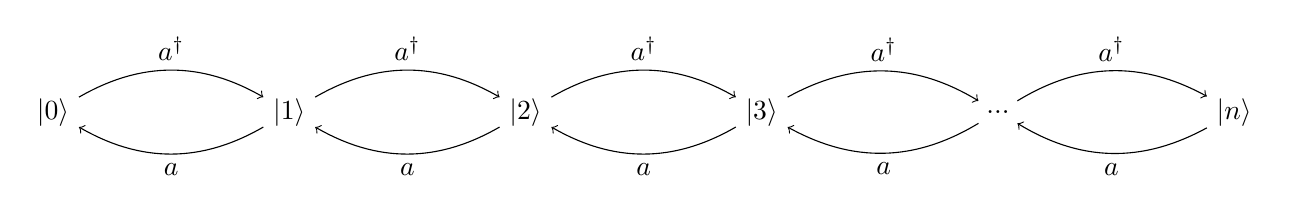
\begin{tikzpicture}
    \node (A) at (0, 0) {$|0 \rangle $};
    \node (B) at (3, 0) {$|1 \rangle $};
    \draw[->, bend left] (A) to node[above] {$a^\dag$} (B);
    \draw[->, bend left] (B) to node[below] {$a$} (A);
       \node (C) at (6,0) {$| 2 \rangle$};
    \draw[->, bend left] (B) to node[above] {$a^\dag$} (C);
    \draw[->, bend left] (C) to node[below] {$a$} (B);
    \node (D) at (9,0) {$| 3 \rangle$};
    \draw[->, bend left] (C) to node[above] {$a^\dag$} (D);
    \draw[->, bend left] (D) to node[below] {$a$} (C);
    \node (E) at  (12,0) {...};
    \draw[->, bend left] (D) to node[above] {$a^\dag$} (E);
    \draw[->, bend left] (E) to node[below] {$a$} (D);
    \node (F) at (15,0) {$|n\rangle$};
    \draw[->, bend left] (E) to node[above] {$a^\dag$} (F);
    \draw[->, bend left] (F) to node[below] {$a$} (E);
\end{tikzpicture}
\vspace{1cm}

\noindent In conclusione abbiamo che l'energia dell'oscillatore armonico \`e quantizzata e non pu\`o assumere valori arbitrati. Il valore pi\`u piccolo che pu\`o assumere (stato fondamentale) \`e dato da 
\begin{equation*}
	E_0 = \frac{\hbar \omega}{2}
\end{equation*}

\subsubsection{Autostati della Hamiltoniana }

Il vettore $|0\rangle $ associato a $n=0$ soddisfa la condizione 
\begin{equation*}
	a |0 \rangle = 0 
\end{equation*}
Essendo definito da una fattore costante, possiamo assumere che $|0 \rangle $ sia normalizzato e che la sua indeterminazione sia associata solo a un fattore di fase $e^{i\theta}$, per $\theta \in \mathbb{R}$. Per le prorpiet\`a viste sull'
operatore di innalzamento abbiamo che in generale
\begin{equation}
	a^\dag |n\rangle = c_n |n+1 \rangle
\end{equation}
dove 
\begin{align*}
	& \|a^\dag | n \rangle \|^2 = \langle n | a^\dag a | n \rangle = \langle n| a^\dag a +1 | n \rangle = \langle n| n+1 |n \rangle =n+1 \langle n | n \rangle = n+1 =\\[0.5cm]
	& =\|c_n|n+1 \rangle \|^2 = |c_n|^2\||n+1 \rangle \|^2 = |c_n|^2 \\[0.5cm]
	& \Rightarrow |c_n| = \sqrt{n+1}
\end{align*}
e quindi l'uguaglianza (3.29) diventa 
\begin{equation}
	a^\dag |n \rangle = \sqrt{n+1}|n+1 \rangle 
\end{equation}
con analogo procedimento possiamo definire l'operatore di abbassamento
\begin{equation*}
	a|n\rangle = \sqrt{n}|n-1 \rangle 
\end{equation*}
dalla relazione (3.30) possiamo definire la forma degli autostati in funzione dell'operatore $a^\dag$, infatti
\begin{equation*}
	|n + 1 \rangle = \frac{1}{\sqrt{n+1}}a^\dag |n \rangle 
\end{equation*}
e dato che gli autostati insieme agli operatori $a$ e $a^\dag$ definiscono una scala di stati questi sono legati tra loro dall'applicazione degli operatori in modo iterativo, arrestandosi allo stato fondamentale. Se consideriamo
\begin{equation*}
	|n \rangle = \frac{1}{\sqrt{n}}a^\dag |n-1 \rangle 
\end{equation*} 
reiterando sull'autostato $|n-1 \rangle $ l'espressione diventa
\begin{equation*}
|n \rangle = \frac{1}{\sqrt{n}} \frac{1}{\sqrt{n-1}}a^\dag |n-2 \rangle
\end{equation*}
procedendo fino allo stato fondamentale otteniamo che l'autostato $|n \rangle$ generico per un oscillatore armonico pu\`o essere espresso come 
\begin{equation}
	|n \rangle = \frac{1}{\sqrt{n!}}(a^\dag)^n|0\rangle 
\end{equation}
In teoria dovremmo verificare che le autofunzioni cos\`i definite siano una base ortonormale del sottospazio di Hilbert, ma dato che H per ipotesi \`e Hermitiana ed \`e un osservabile , possiamo concludere che gli elementi $|n\rangle$ sono ortonormali ta loro e quindi l`insieme delle autofunzioni \`e una base del sottinsieme $\mathcal{E}_{x}$.


\subsubsection{La funzione d'onda}

Per determinare la forma funzionale delle autofunzioni senza risolvere l'equazione di Schr\"odinger introduciamo un cambio di coordinate definendo le grandezze 
\begin{equation*}
	\hat{x} = \sqrt{\frac{m \omega }{\hbar}}\hat{\xi}
\end{equation*}
rispettivamente rispetto ai momenti e coordinate 
\begin{align*}
	& \hat{X} = \sqrt{\frac{\hbar}{m\omega}}\hat{x}  \to \hat{X} = \hat{\xi} \\[0.5cm]
	& \hat{P} = \frac{-i \hbar }{\sqrt{m\omega \hbar}}  \hat{p} = \frac{-i \hbar }{\sqrt{m\omega \hbar}} \frac{d}{dx} \to -i \frac{d}{d\xi}
\end{align*}

nell'ultimo passaggio si \`e richiesto che la trasformazione rispetto a $\hat{x}$ fosse invertibile e dunque si \`e applicata la regola 
\begin{equation*}
	\frac{d}{dx} = \frac{d \xi}{dx} \frac{d}{d\xi} = \sqrt{\frac{m \omega }{\hbar}} \frac{d}{d \xi }
\end{equation*}
Dalla relazione (3.31) sappiamo che la forma esplicita degli autostati \`e legata a quella dello stato fondamentale, di conseguenza partendo dall'equazione
\begin{equation*}
	a | 0 \rangle = 0 \iff \frac{1}{\sqrt{2}}(\hat{X}+i \hat{P})|0\rangle  = 0 
\end{equation*}
e utilizzando le trasformazioni definite in precedenza otteniamo l'equazione differenziale
\begin{equation*}
	\left ( \frac{d}{d\xi} + \xi \right)|0 \rangle = 0 \iff \frac{d|\psi_0(\xi) \rangle }{d\xi} = -\xi|\psi_0(\xi) \rangle 
\end{equation*}
essendo una EDO del primo ordine questa \`e risolubile per quadrature e dunque
\begin{equation*}
	|\psi_0 (\xi)\rangle = A e^{-\xi^2/2} 
\end{equation*}
Imponendo la condizione di normalizzazione determiniamo il coefficiente A.
\begin{align*}
	& 1 = \int_{\mathbb{R}}d\xi \;  |\psi_0(\xi)|^2 = \int_{\mathbb{R}}d\xi \; |A|^2 e^{-\frac{m\omega}{\hbar}x^2} = |A|^2 \sqrt{\frac{\pi \hbar^2}{m \omega}}\\[0.5cm]
	& \Rightarrow A = \left (\frac{m\omega}{\pi \hbar^2}\right)^{1/4}
\end{align*}
e quindi la funzione d'onda dello stato fondamentale \`e data da 
\begin{equation}
	|\psi_0 (x)\rangle = \left (\frac{m\omega}{\pi \hbar^2}\right)^{1/4} e^{-\frac{m\omega}{\hbar}x^2}
\end{equation}
\newpage

\noindent sostituendo nella relazione (3.31) abbiamo che un generico stato $|n \rangle$ \`e esprimibile come
\begin{align*}
	|\psi_n(\xi)\rangle = & \frac{1}{\sqrt{n!}} (a^\dag)^n|\psi_0(\xi) \rangle = \\[0.5cm]
	=& \frac{1}{\sqrt{n!2^n}} \left( \xi - \frac{d}{d\xi} \right )^n \left ( \frac{m\omega}{\pi \hbar} \right)^{1/4} e^{-\xi^2/2} = \\[0.5cm]
	= & \left ( \frac{m\omega}{\pi \hbar} \right)^{1/4}\frac{H_n(\xi)}{\sqrt{n!2^n}} \; e^{-\xi^2/2}
\end{align*}
dove il termine $H_n(\xi)$ definisce un \textit{polinomio Hermitiano}. Dunque la soluzione generale di un oscillatore armonico \`e costituita da un termine esponenziale moltiplicato per un polinomio. Di seguito riportiamo un grafico delle prime quattro funzioni d'onda e i valori del polinomio di Hermite.

\begin{align*}
	&H_0(\xi) = 1\\[0.2cm]
	&H_1(\xi) = 2 \xi\\[0.2cm]
	&H_2(\xi) = 4\xi^2\\[0.2cm]
	&H_3(\xi) = 8\xi^3 - 12\xi
\end{align*}

 
\begin{figure}[!ht]
\vspace{0.1in}
\includegraphics[width = 13cm]{waveOscillatore}	
\centering
\vspace{0.1in}
\caption{Funzione d'onda normalizzate. Scorrendo da sinistra verso destra si passa dallo stato fondamentale al terzo stato eccitato.}
\end{figure}

Notare come al crescere di $n$ crescono le intersezioni con l'asse delle ascisse da parte della funzione d'onda  $|n \rangle $, questo vuol dire che il valore medio dell'energia potenziale cresce con $n$ e analogamente l'energia cinetica.
\newpage
Quando il numero di zero di $|n \rangle$ aumenta, la curvature della funzione d'onda aumenta e quindi la derivata seconda assume dei valori sempre pi\`u grandi, da qui discende anche il fatto che l'energia  cinetica media aumenta. 

Se prendiamo valori molto grandi di $n$, abbiamo che la densit\`a di probabilit\`a $|\psi_n(x)|^2$ diventa molto grande per $x \simeq x_{max}$, dove $x_{max}$ coincide con il punto d'inversione (dove l'energia cinetica si annulla) di una particella nella trattazione classica dell'oscillatore armonico. Mediamente, una particella spende pi\`u tempo in un intorno dei punti d'inversione che al centro dell'intervallo $-x_{max} \leq x \leq x_{max}$.

 
\begin{figure}[!ht]
\vspace{0.1in}
\includegraphics[width = 15cm]{waven}	
\centering
\vspace{0.1in}
\caption{Funzioni d'onda di un oscillatore armonico per il $20^{th}$} stato eccitato sulla sinistra, e il $60^{th}$ stato eccitato sulla destra.
\end{figure}

\subsubsection{Propriet\`a del polinomio di Hermite }

Il fatto che gli autostati soluzione dell'oscillatore armonico siano dati dal prodotto di un esponenziale e di un polinomio di Hermite, fa s\`i che queste funzioni siano invarianti rispetto alla trasformazione di Fourier. 
\begin{equation*}
	\psi(p) = e^{i \theta}\psi(x)|_{x = p /m\omega}
\end{equation*}
tale risultato fa s\`i che sotto trasformazione l'equazione di Schr\"odinger trasformata ci restituisce ancora l'equazione di un oscillatore armonico.

I polinomi Hermite sono funzioni o pari o dispari, infatti 
\begin{equation*}
	H_n(-\xi) = (-1)^n H_{n}(\xi)
\end{equation*}
tale propriet\`a ci permette, partendo dalle simmetrie del problema, di determinare la parit\`a o disparit\`a delle soluzioni. 

\section{Oscillatore armonico accoppiato}

Consideriamo una Hamiltoniana della forma 
\begin{equation*}
	H = \frac{p_1^2}{2m} + \frac{p_2^2}{2m} + \frac{m \omega^2}{2}(x_1^2 + x_2^2 + 2 \lambda x_1 x_2)
\end{equation*}

dove l'ultimo termine \`e una forma quadratica, di conseguenza esiste una matrice associata della forma 
\begin{equation*}
\left [ \begin{array}{cc}
		x_1 & x_2\\ 
	\end{array} \right ]
	\underbrace{\left [ \begin{array}{cc}
		1 & \lambda \\ 
		\lambda & 1 
	\end{array} \right ]}_{=Q}
	\left [ \begin{array}{c}
		x_1 \\ 
		x_2 
	\end{array} \right ] 
\end{equation*} 
dato che Q \`e una matrice simmetrica, questa risulta essere diagonalizzabile, ovvero esiste una matrice $R \in SO(3)$ tale per cui possiamo definire Q nel seguente modo 
\begin{equation*}
	Q = R^{T} \left [ \begin{array}{cc}
		q_1 & 0 \\ 
		0 & q_2 
	\end{array} \right ]R
\end{equation*} 
Per risolvere il problema riscriviamo l'equazione di Schr\"odinger dell'oscillatore armonico accoppiato rispetto ad una nuova base. Partendo da
\begin{equation}
	-\frac{\hbar^2}{2m} \left (\frac{\partial^2}{\partial x_1^2} + \frac{\partial^2}{\partial x_2^2} \right) \psi + V(x_1,x_2)\psi = E\psi 
\end{equation} 
definiamo i nuovi elementi della base facendo agire la matrice R $x' = Rx$ e in componenti diventa $x_k' = R_{ks}x_s$. La derivata parziale rispetto alle nuove coordinate diventa 
\begin{equation*}
	\frac{\partial }{\partial x_s} = \frac{\partial x'_k}{\partial x_s}\frac{\partial}{\partial x'_k} = R_{ks} \frac{\partial}{\partial x'_k}
\end{equation*}
in notazione vettoriale si ha che 
\begin{equation*}
	\nabla = R \;\nabla'
\end{equation*}
Riscrivendo (3.33) in forma vettoriale e utilizzando i risultati ottenuti si ha che
\begin{align*}
	&- \frac{\hbar^2}{2m} \nabla^2\psi + (\bold{x}^{T}Q\bold{x}) \psi = E \psi \\[0.5cm]
	&\iff - \frac{\hbar^2}{2m} \nabla^2\psi + (\bold{x}^TR^T\left [ \begin{array}{cc}
		q_1 & 0 \\ 
		0 & q_2 
	\end{array} \right ] \bold{x}R)\psi = E \psi \\[0.5cm]
	& \iff - \frac{\hbar^2}{2m} \left( \nabla' \right)^2 \psi + (\bold{x'}^T\left [ \begin{array}{cc}
		q_1 & 0 \\ 
		0 & q_2 
	\end{array} \right ] \bold{x'})\psi = E \psi
\end{align*}
dove per per il Laplaciano si \`e usata la relazione 
\begin{equation*}
	\nabla^2 = \nabla^T \cdot \nabla = (R\nabla')^T \cdot (R\nabla') = (\nabla')^TR^TR\nabla' = (\nabla')^2  
\end{equation*}
L'equazione di Schr\"odinger nel nuovo sistema di coordinate assume la forma 
\begin{equation*}
	- \frac{\hbar^2}{2m} \left ( \frac{\partial^2}{\partial x_1'^2 } + \frac{\partial^2}{\partial x_2'^2}\right) \psi  + \frac{m\omega^2}{2}\left ( (x_1')^2q_1 + (x_2')^2q_2 \right) \psi = E \psi
\end{equation*}
Studiando il polinomio caratteristico $P(q) = 0$ associato alla matrice (Q - qI) si dimostra che i termini $q_{1}$ e $q_2$ rappresentano le frequenze di oscillazione proprie del sistema.
\begin{equation*}
	det(Q-qI) = \text{det} \left [ \begin{array}{cc}
		1-q & \lambda \\
		\lambda & 1-q 
	\end{array} \right ] = (1-q)^2-\lambda^2 = 0 \Rightarrow q_{1,2} = 1 \pm \lambda
\end{equation*}
Determinato il loro valore esplicito e sostituendo nell'equazione di Schr\"odinger definita rispetto alla nuova base, abbiamo che la Hamiltoniana pu\`o essere interpretata come la somma di due Hamiltoniane che rappresentano rispettivamente un oscillatore armonico con una sua frequenza propria di oscillazione distinta.
\begin{equation*}
	H = H_1 + H_2 = \frac{p_1^2}{2m} + \frac{m\omega^2}{2}(x_1')^2(1+\lambda) + \frac{p_2^2}{2m} + \frac{m \omega^2}{2}(1-\lambda)
\end{equation*}
dove possiamo definire $\omega_1 = \omega \sqrt{1+\lambda}$ per la Hamiltoniana $H_1$ e $\omega_2 = \omega \sqrt{1 -\lambda }$ per la Hamiltoniana $H_2$. Gli autovalori associati al sistema, vista la natura additiva della Hamiltoniana del sistema complessivo, possono essere espressi nel seguente modo 
\begin{equation*}
	H |n \rangle = E_{n}|n \rangle \iff H_1|n\rangle + H_2|n\rangle = E_{n_1}|n \rangle + E_{n_2}|n \rangle  \Rightarrow E_n = E_{n_1} + E_{n_2}  
\end{equation*}
che usando i risultati della sezione precedente, analiticamente assumono la forma
\begin{align*}
	E_{n_1,n_2} = & \hbar \omega_1 \left (n_1 + \frac{1}{2} \right ) + \hbar \omega_2 \left (n_2 + \frac{1}{2} \right ) \\[0.5cm] = 
	& \hbar \omega \sqrt{1+\lambda} \left (n_1 + \frac{1}{2} \right ) + \hbar \omega \sqrt{1-\lambda}\left (n_2 + \frac{1}{2} \right )
\end{align*}

\subsection{Oscillatore armonico in un campo elettrico costante}

Consideriamo una particella di carica $q$ che si muove sotto l'azione di una forza centrale data da un potenziale elettrostatico 
\begin{equation*}
	V(x) = - q \varepsilon x
\end{equation*}
e da una forza di natura elastica, dunque la Hamiltoniana che descrive la dinamica del sistema \`e data da 
\begin{equation*}
	H = \frac{p^2}{2m} + \frac{m\omega^2}{2}x^2 - q\varepsilon x
\end{equation*}
riscriviamo la hamiltoniana nel seguente modo
\begin{equation*}
	H = \frac{p^2}{2m} + \frac{m \omega^2}{2} \left (x - \frac{q \varepsilon}{m \omega^2 }\right)^2 -\frac{q^2\varepsilon^2}{2m\omega^2}
\end{equation*}
effetuando un cambio di variabile
\begin{equation*}
	x' = x - \frac{q\varepsilon}{m \omega^2}
\end{equation*}
in modo tale da avere un oscillatore armonico centrato nell'origine.
\newpage 
\noindent Per quando discusso nei paragrafi precedenti sappiamo che l'energia dell'oscillatore armonico \`e quantizzata e in questo caso specifico, vista la presenza di una costante aggiuntiva nella Hamiltoniana, assume l'espressione 
\begin{equation*}
	E_n = \hbar \omega\left(n + \frac{1}{2} \right ) - \frac{q^2\varepsilon^2}{2m\omega^2}
\end{equation*}
le autofunzioni associate equivalgono a dei polinomi di Hermite traslati.
\begin{equation*}
	\psi_n(x) = Cost \; H_n \left (\alpha \left [x-\frac{q\varepsilon}{m\omega^2} \right ]  \right )e^{-\frac{\alpha^2}{2}\left (x-\frac{q\varepsilon}{m\omega^2} \right )^2} \quad \text{dove} \quad \alpha = \sqrt{\frac{m\omega}{\hbar}}
\end{equation*}
Ipotizziamo di effetuare une sperimento in cui al tempo $t = 0$ non \`e presente nessun campo elettrostatico $\varepsilon = 0$ e il sistema si trova nella configurazione di stato fondamentale $n = 0$ e dunque l'energia \`e al minimo possibile, in un istante  successivo $t > 0$ il campo elettrico viene acceso istantaneamente e quindi $\varepsilon \neq 0$. In condizioni di questo tipo possiamo domandarci: "\textit{Qual \`e la probabilit\`a che il sistema accoppiato resti nello stato fondamentale di partenza ?}
\newline

Per rispondere a questa domanda, ci ricordiamo che un generico stato di un sistema pu\`o essere espresso come combinazioni lineare delle autofunzioni della Hamiltoniana H, dato che queste costituiscono una base ortonormale di un sotto spazio di Hilbert.
\begin{equation*}
	\psi = \sum_{n} c_n \varphi_{n}
\end{equation*}  
Per determinare la probabilit\`a che il sistema di trovi ancora nello stato fondamentale una volta che $\varepsilon \neq 0$ \`e data dal prodotto
\begin{equation}
	|c_0|^2 = \left |\int dx \; (\varphi_0(x)^{\varepsilon \neq 0})^* \; \varphi_0(x)^{\varepsilon = 0} \right | ^2 = P(E = E_0)
\end{equation}
Dai risultati precedenti possiamo definire
\begin{align*}
	& \varphi_0 (x)^{\varepsilon = 0} = \left ( \frac{\alpha^2}{\pi}\right )^{1/4} e^{-\frac{\alpha^2}{2}x^2} \\[0.5cm]
	& \varphi_0(x)^{\varepsilon \neq 0} = \left ( \frac{\alpha^2}{\pi}\right )^{1/4} e^{\frac{\alpha^2}{2}\left (x- \frac{q\varepsilon}{m\omega^2}\right)^2}
\end{align*}
definiamo esplicitamente (3.34) 
\begin{align*}
	P(E=E_0) = &\left ( \frac{\alpha^2}{\pi}\right )^{1/2} \int_{\mathbb{R}}dx \; e^{\frac{\alpha^2}{2}\left (x- \frac{q\varepsilon}{m\omega^2}\right)^2}e^{\frac{\alpha^2}{2}\left (x- \frac{q\varepsilon}{m\omega^2}\right)^2} = \\[0.5cm]
	 = & \left ( \frac{\alpha^2}{\pi}\right )^{1/2} \int_{\mathbb{R}}dx \; e^{- \alpha^2 \left ( x - \frac{q\varepsilon}{2m\omega^2}\right)^2} e^{-\frac{\alpha^2}{2}\frac{q^2\varepsilon^2}{m^2\omega^4} + \frac{\alpha^2 q^2\varepsilon^2}{4m^2\omega^4}} = \\[0.5cm]
	 = & \left ( \frac{\alpha^2}{\pi}\right )^{1/2} \sqrt{\frac{\pi}{\alpha^2}} \; e^{-\frac{\alpha^2}{2}\frac{q^2\varepsilon^2}{m^2\omega^4} + \frac{\alpha^2 q^2\varepsilon^2}{4m^2\omega^4}} = e^{- \frac{\alpha^2}{4}\frac{q^2 \varepsilon^2}{m^2 \omega^4}}
\end{align*}

\section{Moto di una particella carica in un campo elettromagnetico}

Classicamente, la forza esercitata su una particella carica in un campo elettromagnetico \`e descritta dalla \textit{forza di Lorentz}:
\begin{equation*}
	\bold{F} = q(\bold{E} + \bold{v} \times \bold{B})
\end{equation*}
dove $q$ indica la carica e $\bold{v}$ la sua velocit\`a. Le velocit\`a dipendenti dalla forza di un campo magnetico sono leggermente differenti da quelle dovuti ad una forza conservativa data da una potenziale centrale, di conseguenza il passaggio dalla descrizione classica alla descrizione quantistica, sostituendo posizioni e momenti con gli opportuni operatori, risulta essere pi\`u delicato di quanto visto nelle casistiche precedenti.

\subsection{Descrizione classica di una particella in un campo}

Dato che la forza di Lorentz dipende dalla velocit\`a, non pu\`o essere espressa come gradiente del potenziale. Inoltre il cammino che compie la particella carica deve essere descrivibile dal principio di minima azione. Dato che $\bold{E}(\bold{r},t)$ e $\bold{B}(\bold{r},t)$ sono legate tra loro dalle equazioni di Maxwell, possiamo introdurre il potenziale scalare $U(\bold{r},t)$ e il \textit{potenziale vettore} $\bold{A}(\bold{r},t)$, in questo modo 
\begin{equation*}
	\left \{ \begin{array}{l}
		\bold{E}(\bold{r},t) = - \nabla U(\bold{r},t) - \frac{\partial}{\partial t}\bold{A}(\bold{r},t)\\[0.5cm]
		\bold{B}(\bold{r},t) = \nabla \times \bold{A}(\bold{r},t)
	\end{array}\right.
\end{equation*}
Quando effettuiamo una trasformazione di questo tipo, diciamo che si \`e effettuata una \textit{trasformazione di Gauge}. Notare che per una trasformazione di questo tipo il campo magnetico ed elettrico non sono univocamente determinati da $\bold{A}$ ed $U$, possiamo avere 
	valori differenti di $\bold{A}'$ e $U'$ che descrivono il medesimo campo.

Essendo la trasformazione di Gauge una ridondanza della descrizione fisica del campo elettromagnetico, poich\`e non \`e altro che una sua parametrizzazione mediante $\bold{A}$ e $U$ (che sono grandezze senza un reale significato fisico), si ha dunque che le grandezze fisiche dipendenti da tali quantit\`a restano invariate. Si dice che sia la meccanica classica che quella quantistica sono \textit{invarianti per Gauge}.
	
La  Lagrangiana corrispondente al sistema parametrizzato \`e data da
\begin{equation*}
	\mathcal{L} = \frac{1}{2}m \bold{v}^2 - qU + q\bold{v} \times \bold{A} 
\end{equation*}
per definire la Hamiltoniana del sistema definiamo i momenti canonici 
\begin{equation}
	p_i = \frac{\partial \mathcal{L}}{\partial \dot{x}_i} = mv_i + qA_i
\end{equation}
in cui compare un termine aggiuntivo al prodotto tra massa e velocit\`a. 
\newpage
 
Dato che la Hamiltoniana per definizione \`e la trasformata di Legendre della Lagrangiana si ha che
\begin{equation*}
	H(q_i,p_i) = \sum_{i}(mv_i + qA_i)v_i - \frac{1}{2}m\bold{v}^2+ qU - q \bold{v} \cdot \bold{A} =  \frac{1}{2}m\bold{v}^2 + qU 
\end{equation*}
che possiamo riscrivere in forma compatta rispetto ai momenti generalizzati come 
\begin{equation*}
	H = \frac{1}{2m}(\bold{p} - q \bold{A}(\bold{r},t))^2+ qU(\bold{r},t)
\end{equation*}
Consideriamo ora le equazioni di Hamilton del moto 
\begin{equation*}
	\left \{ \begin{array}{l}
		\dot{x}_i = \frac{\partial H }{\partial p_i} \\
		\dot{p}_i = -\frac{\partial H}{\partial x_i}
	\end{array}\right.
	\iff 
		\left \{ \begin{array}{l}
		\dot{x}_i = \frac{1}{m} (p_i - qA_i)\\
		\dot{p}_i = -\frac{1}{m}(p_j-qA_j)\left ( -q \frac{\partial A_j}{\partial x_i}\right)-q\frac{\partial U}{\partial x_i} = \frac{1}{m}\dot{x}_j \left (q \frac{\partial A_j}{\partial x_i} \right) - q \frac{\partial U}{\partial x_i}
	\end{array}\right.
\end{equation*}	
La prima equazione determina l'espressione per il momento canonico, mentre la seconda ci riconduce alla forza di Lorentz. Per capire in quale modo, procediamo nel calcolare la derivata prima dei momenti coniugati in (3.35):
\begin{align*}
	m\ddot{x}_i = & \; \dot{p}_i - \frac{d A}{d t} =  \dot{x}_j \left (q \frac{\partial A_j}{\partial x_i} \right) - q \frac{\partial U}{\partial x_i} - q \frac{\partial A}{\partial t} - q \frac{\partial A_i}{\partial x_j}\dot{x}_j = \\[0.5cm]
	= & \; - q \left ( \frac{\partial U}{\partial x_i} - \frac{\partial A_j}{\partial t} \right) + q \dot{x}_j \left (\frac{\partial A_j}{\partial x_i} - \frac{\partial A_i}{\partial x_j} \right) = \\[0.5cm]
	= & \; qE_i +q  \varepsilon_{ijk}\dot{x}_jB_k = qE_i + q (\dot{\bold{x}} \times \bold{B})
\end{align*}
In questo modo otteniamo l'espressione della forza di Lorentz.

\subsection{Descrizione quantistica di una particella in un campo}

Per passare alla trattazione quantistica, come sempre sostituiamo la quantit\`a di moto con la il suo analogo operatore $ \hat{\bold{p}} = - i \hbar \nabla $. In questo $\hat{p_i} \neq  m \hat{v}_i$, di conseguenza avremo che le velocit\`a in direzioni differenti non commutano. L'operatore associato all'osservabile della Hamiltoniana viene definito come 
\begin{equation*}
	\hat{H} = \frac{1}{2m} \left ( - i\hbar\nabla - q\bold{\hat{A}} \right)^2 - qU 
\end{equation*}
 L'operatore 
\begin{equation*}
	(\hat{p} - q \hat{A})^\dag = (\hat{p} - q \hat{A}) 
\end{equation*}
\`e un operatore autoaggiunto.
L'equazione di Schr\"odinger associata al sistema \`e definita nel seguente modo
\begin{equation}
	i\hbar \frac{\partial \psi }{\partial t} = \frac{1}{2m} (-i\hbar \nabla - qA)^2 \psi + qU\psi 
\end{equation}
L'equazione dipende dalla scelta dei potenziale vettoriale e del potenziale scalare, dove entrambi possono essere definiti arbitrariamente. Per questo motivo l'informazione restituita dall'equazione (3.36) deve essere invariante rispetto alla scelta di $A$ e $U.$ 
\newpage 

Per dimostrarlo partiamo dai parametri A e U e consideriamo la loro trasformazione 
\begin{equation}
	\left \{\begin{array}{l}
		U' = U - \frac{\partial \Lambda}{\partial t} \\ 
		A' =  A - \nabla \Lambda \\
	\end{array}\right.
\end{equation}

dove il termine $\Lambda$ prende il nome di \textit{funzione di Gauge}. Dalla seconda equazione avremo che il campo magnetico $\bold{B}$ rimane invariato, ma non quello elettrostatico $\bold{E}$, ma utilizzando la prima trasformazione in (3.37) ovviamo a questo problema. Dato che la Hamiltoniana dipende dal vettore potenziale $\bold{A}$ e quindi dipende dalla scelta del gauge, questo ci suggerisce che la funzione d'onda non \`e un invariante rispetto alla trasformazione. La corrispondente trasformazione \`e data da 
\begin{equation}
	\psi'(\bold{r},t) = \exp \left [i \frac{q}{\hbar} \Lambda(\bold{r},t) \right ]\psi(\bold{r},t)
\end{equation}

La trasformazione di gauge introduce un termine aggiuntino di fase alla funzione d'onda di partenza. Per dimostrare l'invarianza dell'equazione (3.36) osserviamo anche che i momenti $p_i$ sono invarianti rispetto alla trasformazione di gauge e introduciamo il risultato intermedio 
\begin{align*}
	(\hat{p}'_i - qA'_i)e^{\frac{i}{\hbar}q \Lambda } = & \;e^{\frac{i}{\hbar}q \Lambda}(\hat{p}_i-qA'_i) + [\hat{p}_i-qA_i,e^{\frac{i}{\hbar}q\Lambda}]  = \\[0.5cm]
	=& \; e^{\frac{i}{\hbar}q\Lambda}(\hat{p}_i-qA'_i) + q \frac{\partial \Lambda}{\partial x_i}e^{\frac{i}{\hbar}q\Lambda} = \\[0.5cm]
	= & \; e^{\frac{i}{\hbar}q\Lambda}\left (\hat{p}_i-qA'_i + q\frac{\partial \Lambda}{\partial x_i} \right) = e^{\frac{i}{\hbar}q\Lambda}(\hat{p}_i - qA_i)   
\end{align*}
Partendo dalla trasformazione della funzione d'onda (3.38) e sostituendola in (3.37) avremo che
\begin{align*}
	  & e^{\frac{i}{\hbar}q\Lambda} \left ( i \hbar \nabla - q \frac{\partial \Lambda}{\partial t}\right)\psi = \frac{1}{2m}e^{\frac{i}{\hbar}q\Lambda}(\hat{\bold{p}}-q\bold{A}'_i)^2 \psi + q e^{\frac{i}{\hbar}q\Lambda}\left ( U - \frac{\partial \Lambda}{\partial t}\right) \psi  \iff \\[0.5cm]
	  & \iff i \hbar \frac{\partial \psi}{\partial t} = \frac{1}{2m} (\hat{p} -qA)^2\psi +qU\psi
\end{align*}
e dunque l'equazione di Schr\"odinger risulta essere invariante per trasformazione di gauge.

Osserviamo  che il termine di fase introdotto in (3.38) sulla trasformazione della funzione d'onda non influisce sulla densit\`a di probabilit\`a, infatti
\begin{equation*}
	|\psi(\bold{r},t)|^2 =|\psi'(\bold{r},t)|^2
\end{equation*}
di conseguenza cambia l'espressione della funzione d'onda, ma rimane immutata l'informazione fisica contenuta.

\subsection{Particella in campo magnetico costante}

Consideriamo la Hamiltoniana 
\begin{equation*}
	H = \frac{1}{2m} (\bold{p}-q\bold{A})^2 + qU = \frac{1}{2m}\bold{p}^2 - \frac{q}{2m}(\bold{p} \cdot \bold{A} + \bold{A} \cdot \bold{p}) + \frac{q^2}{2m}\bold{A}^2 + qU
\end{equation*}
\newpage
scegliamo un gauge affinch\`e $\nabla \cdot \bold{A} = 0$, tale condizione in meccanica quantistica si traduce nel richiedere che 
\begin{equation*}
	\sum_{i}^3 [p_i,A_i] = - i \hbar \left ( \frac{\partial A_1}{\partial x_1} + \frac{\partial A_2}{\partial x_2} + \frac{\partial A_3}{\partial x_3}\right) = - i\hbar \nabla \cdot \bold{A} = 0
\end{equation*}
e quindi che $[\bold{p},\bold{A}] = 0$. La Hamiltoniana assume la forma 
\begin{equation}
	H = \frac{1}{2m} \bold{p}^2 -\frac{q}{m} \bold{p} \cdot \bold{A} + \frac{q^2}{2m}\bold{A} + qU
\end{equation}
Scegliamo un potenziale vettore $\bold{A}$ affinch\`e venga preservata la condizione sulla sua divergenza e il campo magnetico $\bold{B}$ resti costante, per farlo risolviamo il sistema di equazioni alle derivate parziali 
\begin{equation*}
	\left \{ \begin{array}{l}
		\bold{B} = \nabla \times \bold{A} \\
		\nabla \cdot \bold{A} = 0
	\end{array}\right.
\end{equation*}
che ha come soluzione  
\begin{equation*}
	\bold{A} = -\frac{1}{2} \bold{x} \times \bold{B}
\end{equation*}
Il prodotto scalare tra momenti coniugati e potenziale vettore presenti nella Hamiltoniana possono essere riscritti in funzione della soluzione, calcolando
\begin{equation*}
	\bold{p} \cdot \bold{A} = \sum_i p_iA_i = \sum_i\frac{1}{2}p_i \varepsilon_{ijk}x_jB_k = \sum_i\frac{1}{2} \varepsilon_{ijk}p_ix_jB_k = \sum_i \frac{B_k}{2}\varepsilon_{ijk}x_jp_i = \sum_k\frac{B_k}{2}(\bold{x} \times \bold{p})_{k} = \frac{1}{2} \;\bold{B} \cdot \bold{L}
\end{equation*}
e quindi ottenendo 
\begin{equation*}
	H = \frac{\bold{p}^2}{2m} - \frac{q}{2m}\bold{B} \cdot \bold{L} + \underbrace{\frac{q^2}{8m}|\bold{x} \times \bold{B}|^2}_{(I)} + qU
\end{equation*}
Se $\bold{B}$ \`e sufficientemente piccolo il termine (I) \`e trascurabile e quindi 
\begin{equation*}
	H = - \vec{\mu} \cdot \bold{B}
\end{equation*}
dove il termine $\vec{\mu}$ rappresenta il \textit{momento magnetico}. Ogni volta che una particella possiede un momento angolare, il momento magnetico fornisce un contributo al moto rotazionale dato che $\vec{\mu} = \gamma \bold{L}$, dove $\gamma$ \`e il \textit{fattore giromagnetico}.

Nella formulazione ridotta della Hamiltoniana (in cui trascuriamo (I)) abbiamo che il fattore giromagnetico coincide con $\gamma = q /2m$, per un elettrone vista la dipendenza dalla carica avremo che $\gamma <0$. Per eliminare la dipendenza dal segno della carica possiamo definire 
\begin{equation*}
	\mu_B = \frac{|q|\hbar}{2m}
\end{equation*}
che prende il nome di \textit{magnetone di Bohr}. Nel sistema internazionale la sua unit\`a di misura \`e data da $\mu_b \simeq 9 \times 10^-24 \;  J/T $.
\newpage 
\subsection{Effetto Zeemann}

Consideriamo un elettrone di una atomo idrogenoide, che si muove in un potenziale Coulombiano e in presenza di un campo magnetico costante, la Hamiltoniana che descrive la dinamica della particella \`e data dall'equazione (3.39). Tale Hamiltoniana possiamo rappresentarla come il contributo di tre Hamiltoniane
\begin{equation*}
	H = H_0 + H_1 + H_2
\end{equation*}
dove rispettivamente 
\begin{align*}
	& H_0 = \frac{\bold{p}^2}{2m} + qU \\[0.3cm]
	& H_1 = -\frac{q}{2m}\bold{B} \cdot \bold{L} \\[0.3cm]
	& H_2 = \frac{q^2}{8m}|\bold{x} \times \bold{B}|^2 
\end{align*}
Dove $H_1$ viene definito \textit{termine paramagnetico} e $H_2$ termine \textit{diamagnetico}. Se scegliamo l'orientazione campo magnetico lungo l'asse $z$ l'ultimo termine assume la forma
\begin{equation*}
	H_2 = \frac{q^2B^2}{8m}(x^2+y^2)
\end{equation*}
nel caso degli atomi idrogenoidi possiamo approssimare $\langle x^2 + y^2\rangle \simeq a_0^2$ dove $a_0$ \`e il raggio di Bohr, e $\langle L_z \rangle \simeq \hbar$, di conseguenza il rapporto tra 
\begin{equation*}
\frac{H_2}{H_1} \simeq 10^-6 \quad  B/T 
\end{equation*}
Per i campi ottenibili in laboratorio ($B \simeq 1  \; T$), gli elettroni rimangono legati all'atomo, di conseguenza il termine $H_2$ \`e trascurabile rispetto $H_1$. Se confrontiamo $H_1$ con il potenziale Coulombiano
\begin{equation*}
	\frac{eB\hbar/2m_e}{m_ec^2\alpha^2/2} = \frac{e\hbar}{(m_ec\alpha)^2} \simeq \frac{1}{2.3 \times 10^5} \;\frac{B}{T}
\end{equation*}
dove $\alpha = \frac{e^2}{4\pi \varepsilon_0} \frac{1}{\hbar c} \simeq \frac{1}{137}$ denota la costante di struttura fine; tale risultato ci dice che i termine $H_1$ contribuisce in piccola parte alla perturbazione della classica divisione dello spettro atomico. Considerando quanto discusso fin'ora e tenendo solo il contributo paramagnetico, per un Hamiltoniana "spinless" (definireno lo che cos'\`e lo spin nel capitolo successivo), questa assumer\`a la seguente espressione
\begin{equation}
	\hat{H} = \hat{H_0} + \frac{e}{2m}B_zL_z
\end{equation}
Dato che $[\hat{H}_o,L_z] = 0$, commutano tra loro gli autostati della Hamiltoniana imperturbata $\psi_{lmn}(\bold{r})= R_{n,l}\;(\bold{r})Y_{l}^{m}(\theta,\phi)$ sono anche autostati di $\hat{H}$ e quindi gli autovalori sono dati da 
\begin{equation}
	E_{n,l,m} = -\frac{E_I}{n^2} + m\mu_B B = -\frac{E_n}{n^2} + m\hbar\omega_L
\end{equation}
\newpage 

dove $\omega_L = \frac{eB}{2m}$ indica la \textit{frequenza di Larmor}. Il risultato ci dice che la presenza di un campo magnetico modifica il valore dei livelli di energia associati alla Hamiltoniana $H_0$ per la quale $\bold{B} = 0$, di conseguenza osserviamo un ulteriore divisione di ciascuno dei (2l+1) livelli di energia degeneri associati ad $l$ fissato, separati tra loro per un salto di energia costante $\hbar \omega_L$. Tale fenomeno prende il nome di \textit{effetto Zeemann}.

\begin{figure}[!ht]
\vspace{0.4in}
\includegraphics[width = 13cm]{zeemann}	
\centering
\vspace{0.3in}
\caption{Splitting dei livelli energetici per un elettrone in un campo magnetico costante.}
\end{figure}

\subsection{Livelli di Landau}

Consideriamo una particella carica libera di muoversi sotto l'azione di un campo magnetico costante $\bold{B}(\bold{r})$. Classicamente avremo che la forza di Lorentz esercitata su di essa \`e data da 
\begin{equation*}
	\bold{F} = q\bold{v} \times \bold{B}(\bold{r})
\end{equation*}
dove $\bold{v}$ \`e la velocit\`a della particella. Il moto della particella \`e ovviamente descritto dalla terza (o seconda) legge di di Newton
\begin{equation*}
	m \frac{d^2\bold{x}}{dt^2}= \bold{F}
\end{equation*}
Assumendo che la direzione del campo magnetico sia parallela all'asse $z$, risolvendo l'equazione del moto avremo che che leggi orarie nello spazio della particella sono date da 
\begin{align*}
	&x(t) =x_0 + \sigma \cos (\omega_ct - \varphi_0) \\[0.3cm]
	&y(t) = y_0 + \sigma \sin(\omega_ct - \varphi_0)\\[0.3cm]
	&z(t) = z_0 + v_{0z}t
\end{align*}
\newpage 


dove i termini $x_0,y_0,z_0,\sigma,\varphi_0$ e $v_{0z}$ sono sei parametri costanti determinati dalle condizioni iniziali; il termine $\omega_c$ \`e la \textit{frequenza del ciclotrone} e \`e data da:
\begin{equation*}
	\omega_c = -q \frac{B}{\mu}
\end{equation*}
Le equazioni del moto determinate determinano un moto elicoidale nello spazio, il cui centro \`e dato da $C_0 = C_0(x_0,y_0)$, velocit\`a angolare $\omega_c$ e fase iniziale $\varphi_0$

\begin{figure}[!ht]
\vspace{0.1in}
\includegraphics[width = 7cm]{elycoidal}	
\centering
\vspace{0.1in}
\end{figure}

Per descrivere il campo magnetico $\bold{B}(\bold{r})$, possiamo utilizzare il potenziale vettore $\bold{A}(\bold{r})$ legati tra loro dalla relazione 
\begin{equation*}
	\bold{B}(\bold{r}) = \nabla \times \bold{A}(\bold{r})
\end{equation*}
di conseguenza ripetendo i passaggi visti nelle sezioni precedenti possiamo definire la seguente Lagrangiana
\begin{equation*}
	\mathcal{L}(\bold{r},\bold{v}) = \frac{1}{2}m \bold{v}^2 + q \bold{v} \cdot \bold{A}
\end{equation*}
segue che i momenti coniugati $\bold{p}$ della posizione $\bold{r}$, si legano ad $\bold{A}$ e $\bold{v}$ secondo la relazione
\begin{equation*}
	\bold{p} = \nabla_{\bold{v}}\mathcal{L}(\bold{r},\bold{v}) = m \bold{v} + q \bold{A}(\bold{r})
\end{equation*}
Dunque la Hamiltoniana $H(\bold{r},\bold{p})$ \`e data da:
\begin{equation*}
	H(\bold{r},\bold{p}) = \frac{1}{2m}[\bold{p} - q \bold{A}]^2
\end{equation*}
Un gauge che pu\`o essere utilizzato \`e dato da $\bold{A} = -\frac{1}{2}(\bold{x} \times \bold{B})$, ma questo renderebbe l'equazione di Schr\"odinger pi\`u complicata. Una scelta pi\`u intelligente \`e considerare una direzione privilegiata nel piano (x,y), in questo modo l'equazione di Schr\"odinger coincide con quella di un oscillatore armonico. 

\newpage

Prendiamo un gauge $\bold{A} = (-By,0,0)$. Dato che $\bold{B}$ ha direzione lungo $z$, avremo che la Hamiltoniana diventa 
\begin{equation}
	\hat{H} = \frac{1}{2m}[(\hat{p}_x+qBy)^2 + \hat{p}^2_y + \hat{p}^2_z
\end{equation}
 In questo modo avremo che $\hat{H}$ commuta sia con $\hat{p}_x$ che con $\hat{p}_z$, di conseguenza avremo una base comune di autostati data da 
 \begin{equation*}
 	\psi(x,y,z) = e^{i/\hbar(p_x x+p_z z) }\chi(y)
 \end{equation*}
dove la funzione $\chi(y)$ \`e determinabile sostituendo la soluzione nell'equazione di Schr\"odinger 
\begin{align*}
	& \frac{1}{2m} [ (p_x +qBy)^2 + p_y^2 + p_z^2]\; \chi(y) = E \; \chi(y) \iff\\[0.5cm] 
	& \iff -\frac{p^2_y}{2m}\chi(y) + \frac{q^2B^2}{2m} \left (y + \frac{p_x}{qB} \right)^2\chi(y) + \frac{p_z^2}{2m}\chi(y) = E \; \chi(y) \iff \\[0.5cm]
	& \iff \left[\frac{{\hat{p_y}}^2}{2 m}+\frac{1}{2} m \omega^2\left(y-y_0\right)^2\right] \chi(y)=\left(E-\frac{\hat{p}_z^2}{2 m}\right) \chi(y) 
\end{align*}
dove $y_0 = -p_x / qB$ e $\omega_c$ \`e la frequenza ciclotronica della trattazione classica del moto della carica. Si osserva che il momento coniugato $p_x$ corrisponde alle coordiante del centro di un potenziale che definisce un oscillatore armonico lungo la direzione $y$ con frequenza $\omega_c$.  Di conseguenza, possiamo dedurre che gli autovalori della Hamiltoniana sono dati dati da una componente che descrive il moto libero della carica in direzione parallela al campo, e un insieme stati legati all'oscillatore armonico.
\begin{equation}
	E_{n,p_z} = \hbar \omega_c \left( n + \frac{1}{2} \right) + \frac{p_z^2}{2m}
\end{equation}
Il numero quantico $n$, definisce gli stati che prendono il nome di \textit{livelli di Landau}.

La soluzione dell'equazione di Schr\"odinger \`e data da
\begin{equation}
	 	\psi_{n,p_x,p_z}(x,y,z) = e^{i/\hbar(p_x x+p_z z) }\chi_n(y)\left(y + \frac{p_x}{qB} \right)
\end{equation}

osserviamo che il termine $p_z$ indicizza le autofunzioni, ma non rientra nel valore dell'energia, di conseguenza $p_x \in \mathbb{R}$. Questo vuol dire che esiste un continuo di funzioni d'onda che corrispondono allo stesso livello energetico.

Nelle righe precedenti abbiamo detto che che $p_x$ definisce il centro $y_0$ dell'oscillatore armonico, analiticamente questo \`e dato dalle relazioni
\begin{align*}
	&m\bold{\dot{x}} = \bold{p}-q\bold{A} \iff \bold{p} = m\bold{\dot{x}} + q \bold{A} \\[0.5cm]&\Rightarrow p_z = m\dot{x} - qBy \equiv  -qBy_0
\end{align*}
Il fatto che si abbia la direzione lungo $y$ \`e dato dal motivo che nel gauge si \`e scelta come direzione privilegiata. Se avessimo usato il gauge $\bold{A} = - \frac{1}{2}(\bold{x} \times \bold{B})$, l'equazione di Schr\"odinger avrebbe visto comparire due termini lungo $x$ e $y$ di oscillatore armonico accoppiati con un termine legato al momento angolare.

\noindent I livelli di Landau trovano una grande importanza nella trattazione quantistica dell'effetto Hall.

\section{Esempi ed Esercizi}

\subsection{Esercizio 1: Rotatore rigido}

Consideriamo una particella vincolata a muoversi su una sfera, la sua dinamica \`e descritta dalla Hamiltoniana 
\begin{equation*}
	H = \frac{1}{2I} \bold{L}^2
\end{equation*}
Determinare i valori dell'energia e la loro degenerazione.
\begin{proof}
Per quanto discusso nella sezione di teoria di questo capitolo sappiamo che le equazioni soluzione dell'equazione di Schr\"odinger sono date dalle armoniche sferiche $Y_{lm}(\theta, \phi)$, l'energia associata \`e data dai corrispettivi autovalori che rispetto all'operatore $\bold{L}^2$ sono dati da 
\begin{equation*}
	E_{l} = \frac{\hbar^2 l(l+1)}{2I}
\end{equation*}
per ciascun l fissato, abbiamo che $m = -l,...,0,...,l$ e dunque si hanno $2l+1$ stati associati al medesimo livello energetico.

\end{proof}

\subsection{Esercizio 2}

Consideriamo una particella nello stato iniziale 
\begin{equation*}
	|\psi(x,y,z) \rangle = \frac{\alpha^{\frac{5}{2}}}{\sqrt{\pi}} z e^{-\alpha \sqrt{x^2 + y^2 + z^2}} \quad\; \quad  \alpha > 0 
\end{equation*}
Determinare gli autovalori associati rispetto a $\bold{L}^2$ e $L_z$.
\begin{proof}
Riscriviamo lo stato di partenza rispetto alla basse formata dalla funzioni armoniche 
\begin{equation*}
	|\psi \rangle = C \; Y_{10}re^{-\alpha r} = f(r)Y_{10}(\theta,\phi)
\end{equation*}	
Rispetto ai due operatori abbiamo che 
\begin{equation*}
	\bold{L}^2|\psi \rangle = \hbar^2l(l+1)|_{l=1}|\psi \rangle  = 2 \hbar^2|\psi \rangle  \quad \; \quad L_z|\psi \rangle = \hbar m|_{m=0}|\psi \rangle = 0 
\end{equation*}

\end{proof}

\subsection{Esercizio 3}

Consideriamo una particella nel suo stato fondamentale vincolata in una buca sferica. Determinare la pressione esercitata sulle pareti.
\newpage

\begin{proof}
	La particella \`e soggetta ad un potenziale della forma 
	\begin{equation*}
		V(r) = \left \{ \begin{array}{l}
			0 \quad r \leq R \\
			\infty \quad r > R
		\end{array}\right.
	\end{equation*}
All'interno dell'equazione di Schr\"odinger dobbiamo tenere conto di un termine che descriva la componente del momento angolare della particella a cui \`e soggetta all'interno della buca sferica. Quindi
\begin{equation*}
	-\frac{\hbar^2}{2m}U''(r) + \left ( V(r) + \frac{\hbar^2 l(l+1)}{2mr^2}\right)U = EU
\end{equation*}
Gli stati della particella sono dati dalla soluzione dell'equazione che sono della forma 
\begin{equation*}
	|\psi \rangle = \frac{U(r)_{kl}}{r} Y_{lm}(\theta,\phi)
\end{equation*}
Per evitare problemi al contorno poniamo $U(r) = U(0) = 0$ in modo tale che $U(r) \in L^2(0,+\infty)$. Per richiesta dell'esercizio sappiamo che la particella \`e nel suo stato fondamentale, dunque $l = 0$ e l'equazione di Schr\"odinger diventa
\begin{equation*}
	-\frac{\hbar^2}{2m}U'' = EU \quad r < R
\end{equation*}
che coincide son le equazioni di una particella in una buca infinita, le soluzioni dell'equazione sono date da 
\begin{equation*}
	U_{n0} = \sqrt{\frac{2}{R}} \sin \left( \frac{n\pi r}{R}\right) \quad ; \quad E_{n} = \frac{n^2 \pi^2 \hbar^2}{2mR^2}
\end{equation*} 
Per lo stato fondamentale avremo che $n=1$ e dunque 
\begin{equation*}
		U_{10} = \sqrt{\frac{2}{R}} \sin \left( \frac{\pi r}{R}\right) \quad ; \quad E_{1} = \frac{ \pi^2 \hbar^2}{2mR^2}
\end{equation*}
La forza esercitata dalla particella sulle pareti della buca \`e data da
\begin{equation*}
	F = - \frac{dE_1}{dR} = \frac{\pi^2 \hbar^2}{mR^3} 
\end{equation*}
e quindi la pressione data dal rapporto della forza per unit\`a di superficie \`e equivalente a 
\begin{equation*}
	p = \frac{F}{4\pi R^2} =  \frac{\pi \hbar^2}{4mR^5}
\end{equation*}

\end{proof}

\subsection{Esercizio 4: Effetto Kasimir}

Consideriamo una particella vincolata in una buca sferica di raggio R definita dal  potenziale 
\begin{equation*}
	V(r) = \left \{ \begin{array}{l}
		-V_0 \quad r \leq R \\
		\infty \quad r > R
	\end{array}\right.
\end{equation*} 
\newpage

Per $V_0 > 0$. Trovare il minimo valore di $V_0$ per cui esiste almeno uno stato legato.

\begin{proof}
	Analogamente all'esercizio precedente l'equazione di Schr\"odinger \`e 
\begin{equation*}
	-\frac{\hbar^2}{2m}U''(r) + \left ( V(r) + \frac{\hbar^2 l(l+1)}{2mr^2}\right)U = EU
\end{equation*}	 
Se esiste almeno uno stato legato ci aspettiamo che sia per $l = 0$ e livelli energitici in cui $0 >-E>-V_0$ quindi
\begin{align*}
	& -\frac{\hbar^2}{2m}U''(r)  -V_0 U = EU \quad r < R\\[0.5cm] 
	& -\frac{\hbar^2}{2m}U''(r)  = EU \quad r > R
\end{align*}
Per $r > R$ abbiamo $U = e^{\pm \rho r}$ e per $r < R$ si ha $U(r) = e^{\pm ikr}$ soluzioni delle equazioni precedenti. Gli autovalori associati sono dati da 
\begin{equation}
	E = - \frac{\hbar^2 \rho^2}{2m} \quad ; \quad 
	 E + V_0 = \frac{\hbar^2k^2}{2m}
\end{equation}
Imponendo le condizioni al contorno, dove $U(0) = 0$ avremo che 
\begin{align*}
	U_I(r) = & \; A'e^{ikr} + A''e^{-ikr} = C \cos(kr) + D\sin(kr)  \quad r \leq R \\[0.5cm]
	 & \; \text{Se} \quad  U(0) = 0 \quad  \Rightarrow \quad U_I(r) = D\sin(kr)
\end{align*}
analogamente avremo 
\begin{equation*}
U_{II}(r) = Be^{- \rho r} \quad r > R	
\end{equation*}
Utilizzando le condizioni di raccordo sulla derivata prima definiamo il sistema di equazioni 
\begin{equation*}
	\left \{ \begin{array}{l}
		U_{I}(R) = U_{II}(R) \\
		U_{I}'(R) = U_{II}'(R)
	\end{array}\right. \quad \iff \quad 
	\left \{ \begin{array}{l}
		A \sin(kR) = Be^{-\rho R} \\
		kA \cos(kR) = -\rho Be^{-\rho R}
	\end{array}\right.
\end{equation*}
Dividendo membro a membro abbiamo che 
\begin{equation*}
	\frac{\tan(kR)}{k} = - \frac{1}{\rho} 
\end{equation*}
Dalle relazioni definite in (3.45) otteniamo la relazione $k^2 + \rho^2 = \frac{2mV_0}{\hbar^2}$ e dunque possiamo riscrivere l'uguaglianza precedente come
\begin{equation*}
	\tan(kR) = \underbrace{\frac{-k}{\left [ \frac{2mV_0}{\hbar^2} - k^2\right]^{1/2}}}_{=g(k)}
\end{equation*}
tale equazione non pu\`o essere risolte per via analitica e dunque ricorriamo al metodo grafico.
\newpage
 
\begin{figure}[!ht]
\vspace{0.1in}
\includegraphics[scale = 0.8]{kasimir}	
\centering
\vspace{0.1in}
\caption{}
\end{figure}
In figura abbiamo le due casistiche in cui \`e possibile avere o non avere uno stato legato. Se prendiamo 
\begin{equation*}
	\sqrt{\frac{2mV_0}{\hbar^2}} \geq \frac{\pi}{2R}
\end{equation*}
avremo che la funzione $g(k)$ interseca la funzione tangente in almeno un punto, come si osserva nel primo grafico in figura 3.6. Quindi per rispondere alla domanda del problema, avremo che il valore minimo del potenziale per avere uno stato legato \`e dato da 
\begin{equation*}
	V_0 \geq  \frac{\pi^2 \hbar^2}{8mR^2}
\end{equation*}

\end{proof}

\subsection{Esercizio 5}

Consideriamo una particella di massa $m$ soggetta ad un potenziale elastico e la cui dinamica \`e descritta dalla Hamiltoniana di un oscillatore armonico con frequenza $\omega$. Si trova nello stato iniziale
\begin{equation*}
	\psi(x) = \mathcal{N} \left( 1 + \frac{\alpha x}{2}\right)e^{-\frac{\alpha^2 x^2}{2}} \quad \text{dove} \quad \alpha = \sqrt{\frac{m \omega}{\hbar}} 
\end{equation*}
Determinare:
\begin{enumerate}
	\item La probabilit\`a associata agli stati energetici possibili della configurazione iniziale.
	\item L'evoluto temporale del valore medio della posizione $\langle x \rangle (t)$.
\end{enumerate}

\begin{proof}
1) Per un oscillatore armonico le funzioni soluzione dell'equazione e i rispettivi autovalori sono dati da 
\begin{equation*}
	|n \rangle = \left( \frac{\alpha^2}{\pi} \right)^{\frac{1}{4}} \frac{H_n(\alpha x)}{\sqrt{n!2^n}}e^{-\frac{\alpha^2 x^2}{2}} \quad ; \quad E_n = \hbar \omega \left ( n + \frac{1}{2}\right) \quad n \in \mathbb{N}
\end{equation*}
Riscriviamo la funzione d'onda iniziale rispetto alla base $\varphi_n$, prendendo
\begin{equation*}
	\varphi_0 = C e^{-\frac{\alpha^2 x^2}{2}} \quad \; \quad \varphi_1 = C \; \frac{2 \alpha x}{\sqrt{2}}e^{- \frac{\alpha^2x^2}{2}}
\end{equation*}
\newpage

\begin{equation*}
	\psi(x) = cost \left ( \varphi_0 + \frac{\varphi_1}{2\sqrt{2}}\right) = \sqrt{\frac{8}{9}} \left ( \varphi_0 + \frac{\varphi_1}{\sqrt{8}}\right)
\end{equation*}
La probabilit\`a per gli stati energetici possibili \`e data da 
\begin{equation*}
	P(E=E_0) = \frac{8}{9} \quad \text{e} \quad P(E=E_1) = \frac{1}{9}
\end{equation*}
2) Per calcolare il valore medio della posizione nel tempo, applichiamo  l'operatore di evoluzione temporale 
\begin{equation*}
	\psi(x,t) = \sqrt{\frac{8}{9}} \left (  \varphi_0 e^{-\frac{i}{\hbar}E_0t} + \frac{1}{\sqrt{8}} \varphi_1e^{-\frac{i}{\hbar}E_1t}\right) = \sqrt{\frac{8}{9}} \left ( \varphi_0 e^{-\frac{i\omega t}{2}} + \frac{1}{\sqrt{8}}\varphi_1 e^{-i \frac{3 \omega t}{2}}\right)
\end{equation*}
quindi
\begin{align*}
	\langle x \rangle (t) = & \; \langle \psi |x |\psi \rangle = \int_{\mathbb{R}}dx \;  \psi^*(x,t) \; x \;\psi(x,t)  = \\[0.5cm]
	 = & \frac{8}{9} \int dx \; \left( \frac{1}{\sqrt{8}} e^{-i \omega t}x \; \varphi_0(x)\varphi_1(x) + \frac{1}{\sqrt{8}} e^{i \omega t}x \; \varphi_0(x) \varphi_1(x)\right) = \\[0.5cm] 
	 = & \frac{1}{9 \sqrt{8}}  \; 2 \cos(\omega t) \int_{\mathbb{R}}dx \; x\varphi_0(x) \varphi_1(x) = \frac{4}{9 \alpha} \cos(\omega t)
\end{align*}
dove abbiamo posto a zero i termini $\int dx \; \varphi_0 x \varphi_0$ per parit\`a.

\end{proof}

\subsection{Esercizio 6}

Calcolare i valori medi di posizione $\langle x \rangle $ e momenti $\langle p \rangle$ e le relative incertezze $\Delta x, \Delta y$, per uno stato stazionario dell'oscillatore armonico.
\begin{proof}
Consideriamo i seguenti operatori di posizione e momento
\begin{equation*}
	x = \sqrt{\frac{\hbar}{2m \omega}}(a+a^{\dag}) \quad ; \quad p = i \sqrt{\frac{m\hbar \omega}{2}}(a^{\dag}-a)
\end{equation*}	
Gli stati sono indicizzati da un intero 
\begin{equation*}
	|n \rangle = \frac{(a^{\dag})^n}{\sqrt{n!}}|0 \rangle 
\end{equation*}
per cui valgono le relazioni
\begin{equation*}
	\left \{ \begin{array}{l}
		a^{\dag}|n \rangle = \sqrt{n+1}|n+1 \rangle \\[0.3cm]
		a |n \rangle = \sqrt{n} |n-1 \rangle 
	\end{array}\right.
\end{equation*}
La posizione media \`e data 
\begin{equation*}
	\langle x \rangle = \langle n| x | n \rangle = \sqrt{\frac{\hbar}{2m \omega}} \langle n|a+a^{\dag}|n\rangle =
\end{equation*}
\newpage
\begin{equation*}
	=\sqrt{\frac{\hbar}{2m \omega}}(\langle n|n-1 \rangle \sqrt{n} + \langle n |n+1 \rangle \sqrt{n+1}) = 0
\end{equation*}
Il momento invece 
\begin{equation*}
	\langle p \rangle = \langle n|p|n \rangle = i \sqrt{\frac{m \hbar \omega}{2}} \langle n|a^{\dag} -a|n\rangle = 0
\end{equation*}
Infinite calcoliamo
\begin{align*}
	\langle x^2 \rangle = & \langle n| x^2|n\rangle  = \frac{\hbar}{2m \omega} \langle n| (a+a^{\dag})^2|n\rangle = \frac{\hbar}{2m \omega} \langle n| a^2 + a^{2 \dag} + aa^{\dag} +a^{\dag}a|n\rangle  = \\[0.5cm]
	 = &  \frac{\hbar}{2m \omega} \langle n| aa^{\dag} + a^{\dag}a |n \rangle = \frac{\hbar}{m \omega} \left (n + \frac{1}{2} \right ) 
\end{align*}
e analogamente
\begin{equation*}
	\langle p^2 \rangle = m \hbar \omega \left( n + \frac{1}{2}\right)
\end{equation*}
L'incertezza su momenti e posizioni
\begin{equation*}
	\Delta p^2 = \langle n| p^2|n \rangle = \langle p^2\rangle \quad ; \quad \Delta x^2 = \langle n |x^2|n\rangle = \langle x^2\rangle  
\end{equation*}
Verifichiamo il principio d'indeterminazione  di Heisenberg 
\begin{equation*}
	\Delta x \Delta p = \sqrt{\frac{\hbar}{2m}} \sqrt{m\hbar \omega}\left( n + \frac{1}{2}\right) = \hbar \left(n + \frac{1}{2}\right) \geq \frac{\hbar}{2}
\end{equation*}
Per $n=0$ si ha lo stato stazionario che corrisponde allo stato fondamentale dell'atomo d'idrogeno, in particolare lo stato d'indeterminazione \`e saturato.

\end{proof}

\subsection{Esecizio 7}

Consideriamo una particella di massa $m$ soggetta a un potenziale elastico. La sua evoluzione \`e descritta dall'oscillatore armonico e si trova in uno stato iniziale 
\begin{equation*}
	|\psi(0) \rangle = c_0|0\rangle + c_1|1\rangle 
\end{equation*}
Determinare 
\begin{enumerate}
	\item i coefficienti dello stato iniziale sapendo che $\langle H \rangle = \hbar \omega$ e $\langle x \rangle = \frac{1}{2} \sqrt{\frac{\hbar}{m \omega}}$.
	\item l'evoluto temporale della posizione media nel tempo $\langle x \rangle (t)$.
\end{enumerate}

\begin{proof}
	1) Sappiamo che $P(E=E_0) = |c_0|^2$ e $P(E =E_1)=|c_1|^2$ di conseguenza l'energia media \`e data da 
	\begin{equation*}
		\langle H \rangle = \sum_{n}E_nP(E=E_n) = |c_0|^2E_0 + |c_1|^2E_1 
	\end{equation*}
	e quindi
	\begin{equation*}
		\langle E \rangle = \frac{\hbar \omega}{2}(|c_0|^2+3|c_1|^2) = \hbar \omega
	\end{equation*}
\newpage
poich\`e lo stato sia normalizzato deve valere la condizione $|c_0|^2 + |c_1|^2 =1$. Sostituendo nell'equazione precedente abbiamo che 
\begin{equation*}
	|c_1|^2 = \frac{1}{2} \quad \; \quad |c_0|^1 = \frac{1}{2}
\end{equation*}
Dato che \`e presente un modulo il valore delle costanti \`e definito a meno di un termine di fase e quindi lo stato iniziale in forma generale \`e dato da
\begin{equation*}
	|\psi(0) \rangle = \frac{1}{\sqrt{2}}(e^{i\phi_1}|0 \rangle + e^{i \phi_2}|1\rangle)
\end{equation*}
In meccanica quantistica dato uno stato $|\tilde{\psi} \rangle = e^{i\alpha}|\psi\rangle $ moltiplicato per un numero complesso di modulo 1, la probabilit\`a intrinseca allo stato non cambia. In questo modo \`e possibile cambiare a piacimento le fasi.

2) Definiamo lo stato iniziale come
\begin{equation*}
	|\psi(0) \rangle = \frac{1}{\sqrt{2}}(|0\rangle + e^{i\phi}|1\rangle )
\end{equation*}
e procediamo a calcolare il valore medio della posizione rispetto allo stato iniziale
\begin{align*}
	& \langle x \rangle = \langle \psi(0) |x| \psi(0) \rangle = \frac{1}{2} [\langle 0|x|0\rangle + \langle 1 |x|1\rangle + e^{-\phi}\langle 1|x|0\rangle + e^{i\phi}\langle 0 |x|1\rangle ] = (*) \\[0.5cm]
	& \langle 1|x|0 \rangle = \sqrt{\frac{\hbar}{2m \omega}} \langle 1|a+a^{\dag}|0 \rangle  = \sqrt{\frac{\hbar}{2m \omega}}  \\[0.5cm]
	& \langle 0 |x|1 \rangle = \langle 1|x|0 \rangle^* = \sqrt{\frac{\hbar}{2m \omega}}  \\[0.5cm]
	& (*) = \sqrt{\frac{\hbar}{2m \omega}} \frac{1}{2} (e^{i\phi}+e^{-i\phi}) = \sqrt{\frac{\hbar}{2m \omega}}  \cos(\phi) = \frac{1}{2}\sqrt{\frac{\hbar}{2m \omega}}  \Rightarrow \phi = \frac{\pi}{4}
\end{align*}
quindi lo stato iniziale \`e dato da 
\begin{equation*}
	|\psi(0)\rangle = \frac{1}{\sqrt{2}}(|0\rangle + e^{i \frac{\pi}{4}}|1 \rangle )
\end{equation*}
applicando l'operatore di evoluzione temporale, avremo che il valore medio della posizione al tempo $t$ \`e dato da 
\begin{equation*}
	 \langle x \rangle(t) = \sqrt{\frac{\hbar}{2m \omega}}\cos(\omega t - \frac{\pi}{4}) 
\end{equation*}
Si ottiene una soluzione classica del moto perch\`e l'equazione dei valori medi coincide con quella classica.

\end{proof}

